% =====================================================================
%  Tìm kiếm ảnh ký tự Hán-Nôm tương đồng — bản LaTeX định dạng bài hội nghị
%
%  BIÊN DỊCH:  tectonic -X compile report/paper.tex
%          hoặc  latexmk -xelatex -cd report/paper.tex
%
%  BẮT BUỘC dùng XeLaTeX hoặc LuaLaTeX, KHÔNG dùng pdflatex: bài có chữ Nôm nằm
%  ngoài mặt phẳng cơ bản (U+20000..U+2FFFF) nên phải qua fontspec.
%
%  Hình vẽ sinh bằng `make_figures.py` từ số liệu thật; đừng sửa tay file PDF trong figs/.
%  Sơ đồ trong diagrams/ là TikZ, biên dịch bằng `bash report/diagrams/build.sh`.
% =====================================================================
\documentclass[conference,a4paper]{IEEEtran}

\usepackage{fontspec}
\usepackage{graphicx}
\usepackage{booktabs}
\usepackage{amsmath}
% unicode-math thay cho amssymb: nó cung cấp cả \mathbb/\mathcal VÀ cho phép đặt font toán.
% Không có dòng \setmathfont bên dưới thì phần toán ra Computer Modern trong khi thân bài
% là Termes --- hai kiểu chữ khác nhau trong cùng một câu, thấy rõ nhất ở "$n = 59$".
\usepackage{unicode-math}
\usepackage{array}
\usepackage[hidelinks]{hyperref}
\usepackage{url}

% TeX Gyre Termes = bản Times tự do, phủ đủ dấu tiếng Việt. Gọi theo TÊN FILE chứ không theo tên
% hệ thống ("TeX Gyre Termes"): tên hệ thống cần font được cài vào fontconfig, còn tên file thì mọi
% bản TeX Live / MiKTeX / Tectonic đều tìm được qua kpathsea. Đây là khác biệt giữa "biên dịch được
% trên máy tôi" và "biên dịch được ở mọi nơi".
% Ligatures=TeX để "---" ra gạch dài; CỐ TÌNH không bật cho font mono, nếu không các cờ dòng lệnh
% như --normalize bị nối thành một gạch ngang.
\setmainfont{texgyretermes}[Extension=.otf, UprightFont=*-regular, BoldFont=*-bold,
  ItalicFont=*-italic, BoldItalicFont=*-bolditalic, Ligatures=TeX]
\setsansfont{texgyreheros}[Extension=.otf, UprightFont=*-regular, BoldFont=*-bold,
  ItalicFont=*-italic, BoldItalicFont=*-bolditalic, Ligatures=TeX]
\setmonofont{texgyrecursor}[Extension=.otf, UprightFont=*-regular, BoldFont=*-bold,
  ItalicFont=*-italic, BoldItalicFont=*-bolditalic, Scale=0.86]

\setmathfont{texgyretermes-math.otf}

% Font chữ Nôm. BabelStone phủ phần lớn; HanaMinB phủ Ext-B (chữ Nôm riêng) mà BabelStone thiếu.
% Đã kiểm bằng bảng cmap: mọi ký tự trong bài đều nằm trong font được gán.
\newfontfamily\nomfont{BabelStoneHan.ttf}[Path=../fonts/]
\newfontfamily\nomfontb{HanaMinB.otf}[Path=../fonts/]
\newcommand{\nom}[1]{{\nomfont #1}}
\newcommand{\nomb}[1]{{\nomfontb #1}}
\newcommand{\code}[1]{{\small\texttt{#1}}}

% Việt hoá các nhãn LaTeX tự sinh. Không đặt thì thân bài ghi "Hình 1" trong khi chú thích ghi
% "Fig. 1" — hai ngôn ngữ trong cùng một tham chiếu.
\renewcommand{\figurename}{Hình}
\renewcommand{\tablename}{Bảng}
\renewcommand{\refname}{Tài liệu tham khảo}
\renewcommand{\appendixname}{Phụ lục}

\begin{document}

\title{Tìm kiếm ảnh ký tự Hán-Nôm tương đồng\\
bằng học tương phản trên cặp dương sinh từ font}

\author{\IEEEauthorblockN{Đồ án môn học}
\IEEEauthorblockA{Mã nguồn và toàn bộ lệnh tái lập:
\url{https://github.com/vo-hoang-kh4ng/comparing-character-glyph-images-Sino-N-m}\\
Trọng số: \url{https://huggingface.co/vohoangkh4ng/chinese-clip-ft-sinonom}}}

\maketitle

\begin{abstract}
Báo cáo trình bày một hệ thống tìm những ký tự Hán-Nôm có hình dạng giống với một ảnh chữ cho trước,
trên kho 26.044 ảnh glyph. Nhóm cải thiện hệ thống qua ba bước và đo mọi bước trên cùng một tập
đánh giá. Đầu tiên, nhóm thay bộ trích đặc trưng ResNet18 của bản gốc bằng phần xử lý ảnh của
Chinese-CLIP, nhờ đó chỉ số \code{radical@k} tăng từ 0,2316 lên 0,5361. Tiếp theo, thay vì chỉ dựa
vào các chỉ số gián tiếp, nhóm đo trực tiếp trên 59 ảnh scan thật có nhãn. Kết quả cho thấy mô hình
tốt nhất lúc đó chỉ tìm đúng chữ ở vị trí đầu tiên cho 5/59 ảnh (\code{hit@1} = 0,0847). Cuối cùng,
nhóm tự sinh dữ liệu huấn luyện bằng cách render từng ký tự qua nhiều font rồi làm mờ, làm nhoè cho
giống ảnh scan, sau đó fine-tune mô hình bằng học tương phản có giám sát với nhãn là mã Unicode. Sau
fine-tune, \code{hit@1} trên 59 ảnh scan tăng lên 0,5932 (35/59), và độ chính xác khi xếp hạng trong
nhóm chữ cùng âm Quốc Ngữ tăng từ 0,4746 lên 0,8136. Các ký tự được giữ hẳn ngoài tập huấn luyện cho
kết quả gần như bằng các ký tự đã huấn luyện (0,9939 so với 0,9954), nên mô hình không chỉ học thuộc.
Báo cáo cũng ghi lại hai hướng chưa thành công, một lần huấn luyện bằng ArcFace bị hỏng và tầng xếp
hạng lại bằng siêu dữ liệu, kèm nguyên nhân mà nhóm đo được.
\end{abstract}

\begin{IEEEkeywords}
truy hồi ảnh, chữ Nôm, học tương phản, SupCon, Chinese-CLIP, xếp hạng lại, kết quả âm
\end{IEEEkeywords}

% =====================================================================
\section{Giới thiệu}

Đề bài cho một ảnh chữ Hán-Nôm và yêu cầu tìm trong kho những ký tự có hình dạng gần với nó nhất.
Hệ thống có hai phần, ứng với hai tình huống sử dụng khác nhau. \textbf{Phần 1} tìm trên toàn bộ
26.044 ký tự, dùng khi chưa biết chữ đó đọc là gì, chẳng hạn khi số hoá một trang văn bản chưa được
phiên âm. Đây là tình huống khó. \textbf{Phần 2} dùng khi đã biết cách đọc Quốc Ngữ của chữ: hệ thống
chỉ cần xếp hạng trong nhóm các chữ đọc giống nhau, trung vị khoảng 7 ứng viên, ví dụ khi hiệu đính
một bản phiên âm đã có. Hình~\ref{fig:modes} minh hoạ hai phần trên cùng một ảnh thật, cùng với ba
khó khăn chính của bài toán.

\begin{figure*}[t]
\centering
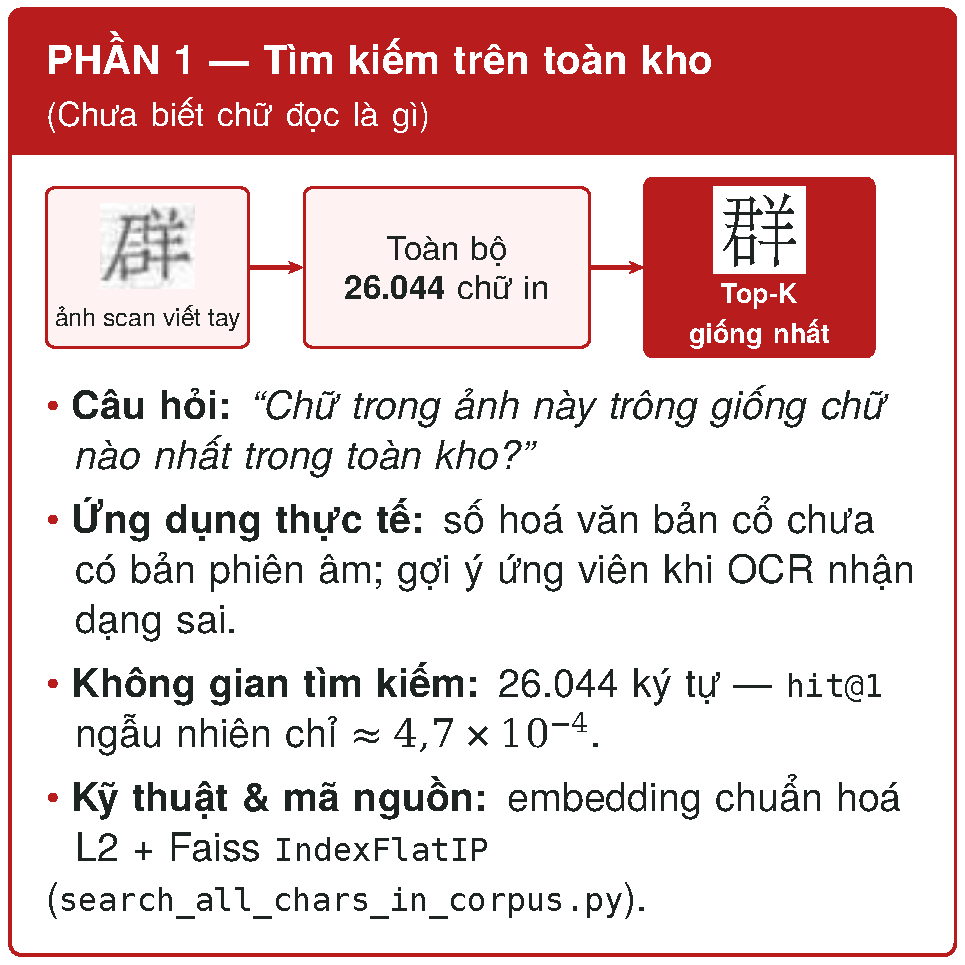
\includegraphics[width=0.495\textwidth]{diagrams/s3-card-phan1.pdf}\hfill
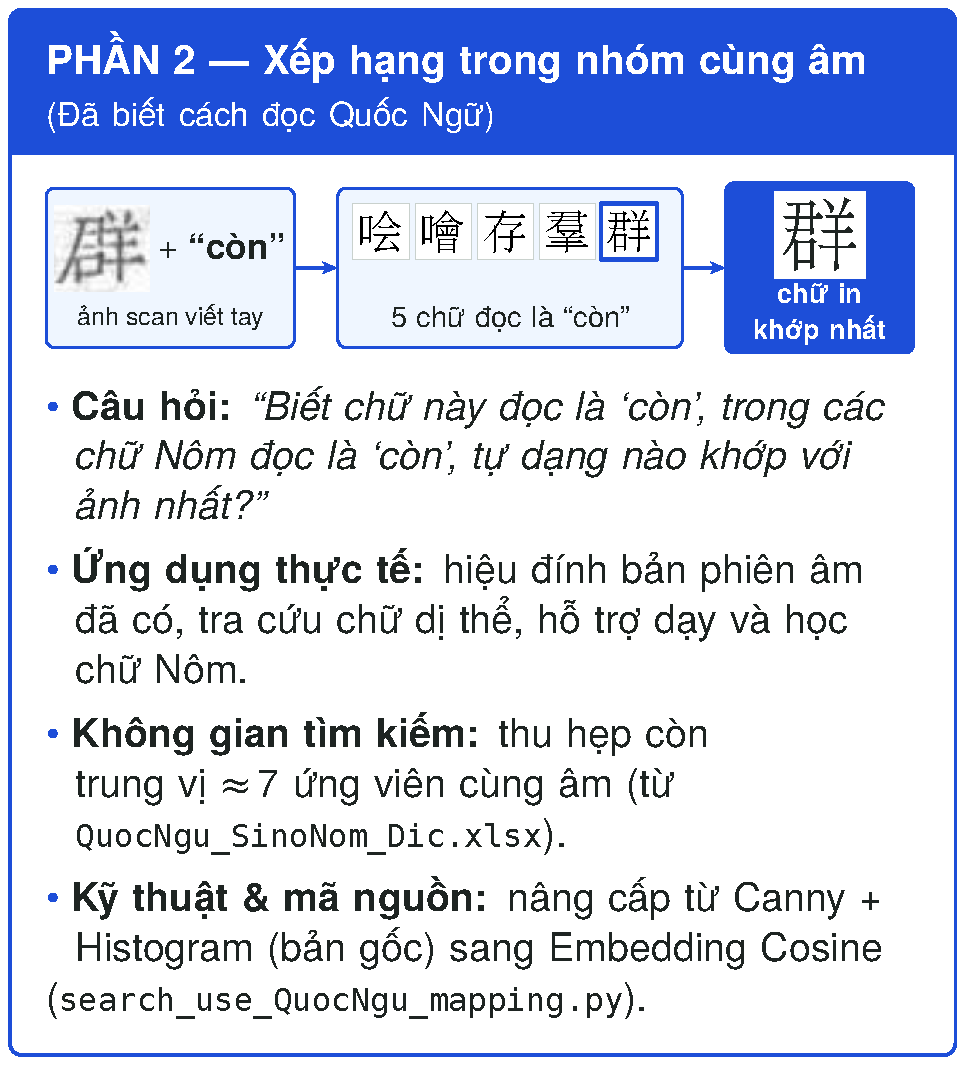
\includegraphics[width=0.495\textwidth]{diagrams/s3-card-phan2.pdf}\\[2mm]

\includegraphics[width=\textwidth]{diagrams/s3-bar-thachthuc.pdf}
\caption{Hai chế độ tìm kiếm trên cùng một truy vấn thật: ảnh scan \code{cofn.jpg} (đọc là ``còn''),
đáp án là \nom{群} (U+7FA4). Ở Phần 2, hệ thống chỉ phải chọn trong 5 chữ đọc là ``còn''. Hàng dưới
là ba khó khăn chính. Chữ \nom{群} trong kho được cắt từ Hình~\ref{fig:qual}; bộ \nom{己已巳} chỉ là ví
dụ minh hoạ.}
\label{fig:modes}
\end{figure*}

Mục~\ref{sec:related} điểm qua các công trình liên quan. Những phần nhóm đã làm được trong đồ án gồm:

\begin{enumerate}
  \item Đánh giá trên \textbf{dữ liệu thật} thay vì chỉ dùng chỉ số gián tiếp: 59 ảnh scan có nhãn,
        kèm mức độ tin cậy do người gán (mục~\ref{sec:eval}).
  \item \textbf{Fine-tune} mô hình (mục~\ref{sec:ft}), nâng \code{hit@1} trên ảnh scan từ 0,0847 lên
        0,5932, và kiểm tra rằng kết quả này không đến từ việc học thuộc (mục~\ref{sec:real},
        \ref{sec:gen}).
  \item Một \textbf{cách sinh dữ liệu huấn luyện} cho kho chỉ có một ảnh mỗi chữ: render chữ qua
        nhiều font, rồi làm suy giảm ảnh theo đúng các số đo lấy từ ảnh scan thật
        (mục~\ref{sec:render}).
  \item Ghi lại đầy đủ các \textbf{kết quả âm}: giới hạn của chính chỉ số \code{radical@k}, một lần
        huấn luyện bị hỏng, và tầng xếp hạng lại chưa đạt kỳ vọng (mục~\ref{sec:neg},
        \ref{sec:rerank}).
\end{enumerate}

Hình~\ref{fig:timeline} tóm tắt quá trình làm đồ án theo từng mốc, mỗi mốc kèm con số đã đo được ở
thời điểm đó.

\begin{figure*}[t]
\centering
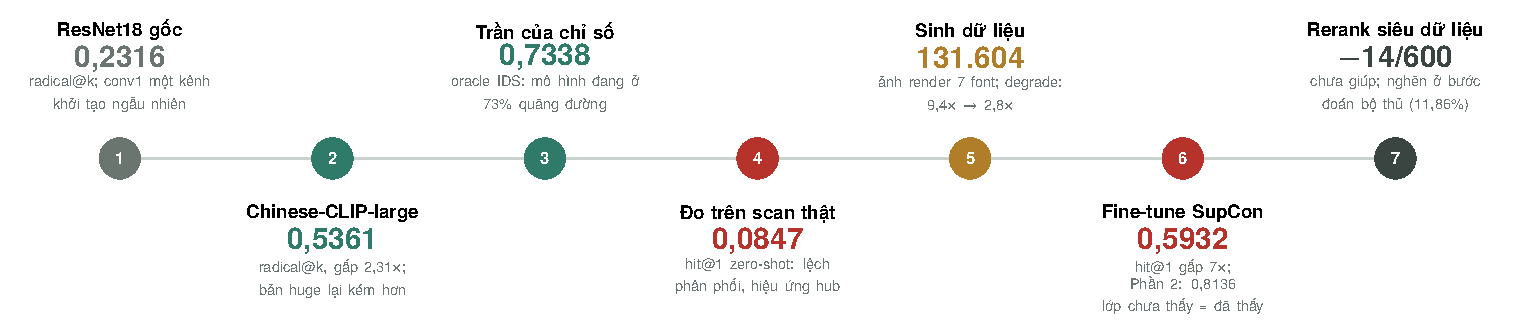
\includegraphics[width=\textwidth]{diagrams/d6-timeline.pdf}
\caption{Các mốc chính của đồ án. Từ mốc 1 đến mốc 3, chỉ số gián tiếp tăng đều. Đến mốc 4, khi đo
trên ảnh scan thật, \code{hit@1} chỉ đạt 0,0847. Mốc 5 và 6 là cách nhóm xử lý kết quả này.}
\label{fig:timeline}
\end{figure*}

% =====================================================================
\section{Công trình liên quan}
\label{sec:related}

\subsection{Mô hình biểu diễn ảnh có sẵn}

Các hệ thống tìm kiếm ảnh hiện nay thường bắt đầu từ một mô hình đã được huấn luyện trước
(pretrain) rồi mới tính đến chuyện huấn luyện thêm. CLIP~\cite{clip} học từ rất nhiều cặp ảnh và
văn bản trên mạng, nên đặc trưng của nó dùng lại được cho nhiều bài toán khác nhau.
Chinese-CLIP~\cite{chineseclip} làm tương tự nhưng trên dữ liệu tiếng Trung, nghĩa là phần xử lý ảnh
của nó đã nhìn thấy rất nhiều chữ Hán khi pretrain. Đây là lý do nhóm chọn Chinese-CLIP thay vì CLIP
gốc. DINOv2~\cite{dinov2} thì học tự giám sát, không cần văn bản. Cả hai đều dùng kiến trúc
ViT~\cite{vit}. Bản gốc của đề bài dùng ResNet18~\cite{resnet} pretrain trên ImageNet; mục~\ref{sec:neg}
cho thấy khoảng cách giữa ResNet18 và Chinese-CLIP không đến từ một chi tiết kiến trúc nhỏ như nhóm
đoán lúc đầu.

\subsection{Học metric và học tương phản}

Học metric có giám sát truyền thống dùng hàm mất mát bộ ba (triplet loss)~\cite{facenet}. Trong thực
tế, điều quan trọng nhất lại là cách chọn ảnh cho mỗi batch: Hermans và cộng sự~\cite{intriplet} chỉ
ra rằng batch phải gồm P lớp, mỗi lớp K ảnh, thì trong batch mới có cặp ảnh cùng lớp để so sánh.
Đây cũng là ràng buộc quan trọng nhất ở mục~\ref{sec:ft}, và bỏ qua nó chính là nguyên nhân của lần
huấn luyện hỏng ở mục~\ref{sec:collapse}.

Học tự giám sát dùng hàm InfoNCE~\cite{infonce}, với cặp dương tạo ra bằng cách biến đổi cùng một
ảnh, như SimCLR~\cite{simclr} và MoCo~\cite{moco}. SupCon~\cite{supcon} kết hợp hai hướng: vẫn dùng
dạng InfoNCE, nhưng coi \emph{mọi} ảnh có cùng nhãn trong batch là cặp dương. Với bài toán này, SupCon
là lựa chọn tự nhiên nhất, vì nhãn (mã Unicode) có sẵn, còn số lớp thì quá lớn để đặt thêm một lớp
phân loại phía trên.

Một hướng khác là softmax có biên góc, tiêu biểu là ArcFace~\cite{arcface}, rất phổ biến trong nhận
dạng khuôn mặt. ArcFace cần học thêm một ma trận tâm lớp kích thước $C \times d$. Trong nhận dạng
mặt, mỗi lớp có hàng chục đến hàng trăm ảnh nên ma trận này học được tốt. Ở bài toán của nhóm
($C = 23.440$ lớp, trung bình 6 ảnh mỗi lớp) thì không, và mục~\ref{sec:collapse} cho thấy hậu quả.
Wang và Isola~\cite{alignuniform} đưa ra một cách kiểm tra đơn giản cho trường hợp này: khi biểu
diễn bị hỏng, các vector dồn lại một chỗ, và có thể phát hiện bằng cosine trung bình giữa các cặp
ngẫu nhiên. Nhóm đã thêm chỉ số này vào vòng đánh giá sau khi gặp sự cố.

\subsection{Sinh dữ liệu bằng render font}

Khi thiếu dữ liệu có nhãn, render chữ bằng font là cách đã được dùng nhiều trong nhận dạng chữ.
Jaderberg và cộng sự~\cite{synth90k} huấn luyện mô hình nhận dạng chữ trong ảnh hoàn toàn bằng dữ liệu
tổng hợp, và Gupta và cộng sự~\cite{synthtext} áp dụng cho bài toán định vị chữ. Cả hai đều nhấn mạnh
rằng ảnh render sạch là chưa đủ, cần làm suy giảm ảnh để nó giống dữ liệu thật hơn. Biến dạng đàn
hồi~\cite{elastic} trong nhận dạng chữ viết tay là một ví dụ quen thuộc. Điểm nhóm làm thêm ở
mục~\ref{sec:render} là chọn tham số suy giảm dựa trên số đo lấy từ chính ảnh scan cần nhận dạng, chứ
không chọn theo cảm tính, và báo cáo luôn khoảng cách còn lại sau khi hiệu chỉnh.

\subsection{Chữ Hán-Nôm}

Chữ Nôm dùng lại các ký tự Hán và thêm nhiều ký tự do người Việt tự tạo. Phần lớn các ký tự này nằm
trong các khối mở rộng của Unicode, có khối nằm ngoài mặt phẳng cơ bản, nên ảnh hưởng đến cả việc
chọn font lẫn cách xử lý chuỗi trong mã nguồn. Ba thông tin thường dùng để tra cứu là bộ thủ, số nét
và cách phân rã chữ thành các bộ phận (IDS, \emph{Ideographic Description Sequence}). Bảng tra của đồ
án có đủ ba trường này, và đây cũng là đầu vào của tầng xếp hạng lại ở mục~\ref{sec:rerank}. Ba trường
này rất tiện để làm chỉ số đánh giá vì có sẵn, nhưng mục~\ref{sec:neg} cho thấy chúng chỉ là nhãn
yếu. Mục~\ref{sec:ft} cũng giải thích vì sao nhóm không huấn luyện trên chúng: nếu huấn luyện trên
một trường rồi lại dùng chính trường đó để chấm điểm thì kết quả không còn ý nghĩa.

% =====================================================================
\section{Dữ liệu}

\begin{table}[t]
\caption{Các tập dữ liệu. Ba tập đầu là dữ liệu đề bài cho; hai tập sau do nhóm tạo hoặc gán nhãn.}
\label{tab:data}
\centering\footnotesize
% Cột p{} mặc định căn đều hai bên, làm chữ giãn xấu trong ô hẹp -> ép raggedright.
\newcolumntype{L}[1]{>{\raggedright\arraybackslash}p{#1}}
\begin{tabular}{@{}L{1.95cm}L{1.75cm}L{3.85cm}@{}}
\toprule
Tập & Kích thước & Vai trò \\
\midrule
\code{images/}      & 26.044 ảnh  & Kho tra cứu. Mỗi ký tự đúng \textbf{một} ảnh. \\
\code{final\_...}    & 31.208 dòng & Bộ thủ, số nét, phân rã IDS. \\
\code{QuocNgu...}   & ---         & Ánh xạ âm Quốc Ngữ $\leftrightarrow$ ký tự. \\
\code{test\_images/} & 59 ảnh scan & \textbf{Tập đánh giá thật}. \\
\code{rendered/}    & 131.604 ảnh & Nhóm sinh ra để huấn luyện, qua 7 font. \\
\bottomrule
\end{tabular}
\end{table}

Bảng~\ref{tab:data} liệt kê các tập dữ liệu. Đặc điểm ảnh hưởng nhiều nhất đến thiết kế là
\textbf{kho chỉ có một ảnh cho mỗi ký tự}. Muốn học cách so sánh hai ảnh, mô hình cần cặp dương, tức
hai ảnh khác nhau của cùng một chữ. Dữ liệu gốc không có cặp nào như vậy, và mục~\ref{sec:render}
trình bày cách nhóm tạo ra chúng.

Ảnh trong \code{test\_images/} được đặt tên theo kiểu gõ Telex (\code{cofn.jpg} là ``còn''). Nhóm
giải mã tên file ra chữ Quốc Ngữ, rồi tra từ điển để lấy \textbf{tập các ký tự đúng} cho ảnh đó. Đây
là nhãn thật chứ không phải nhãn gián tiếp, nên dù chỉ có 59 ảnh, tập này vẫn là căn cứ quan trọng
nhất của đồ án. Hình~\ref{fig:labels} vẽ toàn bộ quá trình lấy nhãn, kể cả hai chỗ nhóm đã phải sửa.

\begin{figure*}[t]
\centering
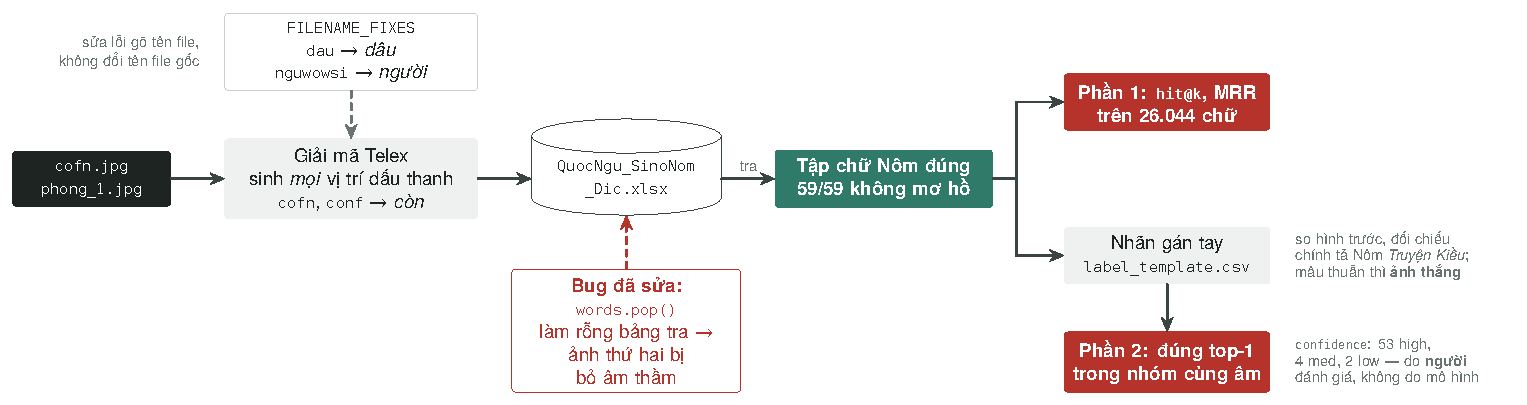
\includegraphics[width=\textwidth]{diagrams/d2-labels.pdf}
\caption{Quá trình lấy nhãn. Tên file Telex được giải mã với mọi vị trí đặt dấu thanh, rồi tra từ
điển để ra tập ký tự đúng cho Phần 1 (59/59 ảnh, không có trường hợp mơ hồ). Phần 2 dùng thêm nhãn do
người gán, kèm mức tin cậy không lấy từ điểm số của mô hình.}
\label{fig:labels}
\end{figure*}

% =====================================================================
\section{Phương pháp}

\subsection{Trích đặc trưng và tìm kiếm}

Mỗi mô hình (gọi là backend) biến ảnh thành một vector và chuẩn hoá L2, nên tích vô hướng giữa hai
vector chính là cosine. Việc tìm kiếm dùng Faiss \code{IndexFlatIP}~\cite{faiss}, tức tìm chính xác,
không xấp xỉ. Bản gốc dùng ResNet18~\cite{resnet} pretrain trên ImageNet, trong đó lớp \code{conv1}
được thay bằng lớp một kênh khởi tạo ngẫu nhiên. Nhóm giữ nguyên bản này để làm mốc so sánh, rồi thêm
năm backend khác: ba kích cỡ của Chinese-CLIP~\cite{chineseclip} và DINOv2~\cite{dinov2}.
Hình~\ref{fig:overview} cho thấy hai phần của hệ thống dùng chung một backend và một bộ vector đã
tính sẵn cho toàn kho.

\begin{figure*}[t]
\centering
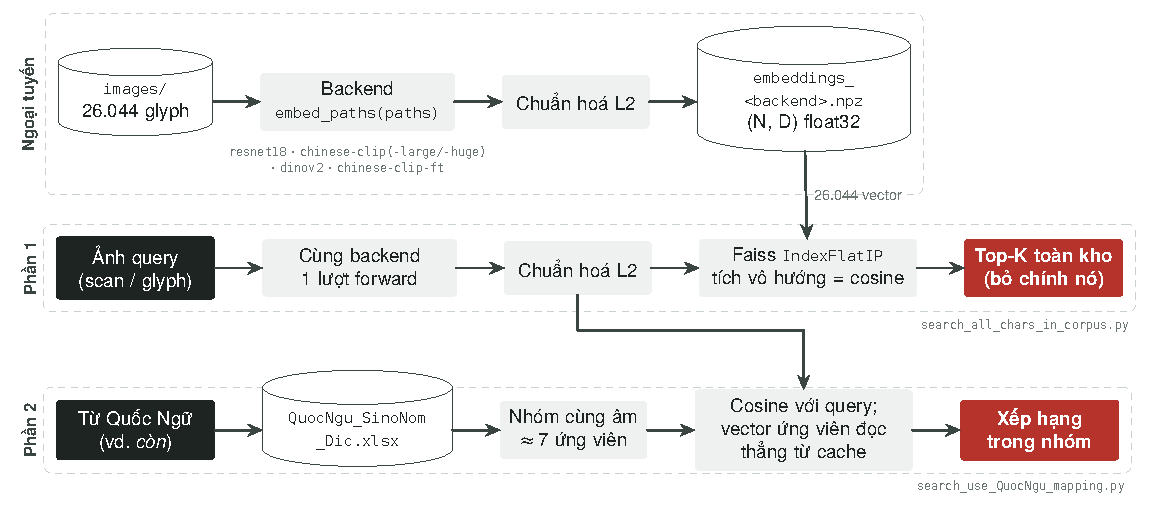
\includegraphics[width=\textwidth]{diagrams/d1-overview.pdf}
\caption{Tổng quan hệ thống. Kho ảnh được trích đặc trưng một lần cho mỗi backend rồi lưu lại. Phần 1
tìm trên toàn bộ 26.044 vector bằng Faiss; Phần 2 chỉ lấy vector của các chữ cùng âm từ bộ đã lưu và
xếp hạng theo cosine.}
\label{fig:overview}
\end{figure*}

\subsection{Sinh cặp dương bằng render nhiều font}
\label{sec:render}

Vì mỗi ký tự chỉ có một ảnh, nhóm render lại từng mã Unicode qua bảy font Hán-Nôm khác nhau. Các ảnh
render của cùng một mã là cùng một lớp nhưng khác kiểu chữ. Trước khi render, nhóm kiểm tra bảng
\code{cmap} của từng font để biết font đó có chứa ký tự hay không; gộp cả bảy font lại thì phủ được
26.033/26.044 ký tự. \textbf{Ký tự nào font không có thì bỏ qua.} Nếu cứ render, font sẽ trả về một ô
vuông rỗng (``tofu'') giống hệt nhau cho mọi ký tự thiếu, và đưa những ảnh đó vào huấn luyện sẽ làm
hỏng cặp dương.

Tuy nhiên ảnh render sạch \emph{quá dễ} so với thực tế. Ảnh render tự tìm lại đúng chữ của nó với
\code{hit@1} = 0,7018, trong khi ảnh scan thật chỉ đạt 0,0847, chênh gần chín lần. Như vậy phần lớn
khoảng cách không nằm ở font. Nhóm đo sáu chỉ số ảnh trên cả hai tập để biết chúng khác nhau ở đâu
(Bảng~\ref{tab:degrade}), rồi viết hàm \code{degrade()} mô phỏng đúng sáu khác biệt đó theo thứ tự
một trang giấy bị scan. Các phép biến đổi này chỉ làm ảnh mờ, nhoè, nhiễu, không làm thay đổi cấu trúc
chữ, nên nhãn vẫn đúng. Sau khi làm suy giảm, \code{hit@1} của ảnh render giảm từ 0,7018 xuống
0,1986, tức chỉ còn dễ hơn ảnh scan thật 2,8 lần thay vì 9 lần. Hình~\ref{fig:synthesis} vẽ toàn bộ
quy trình, gồm cả bước hiệu chỉnh tham số.

\begin{figure*}[t]
\centering
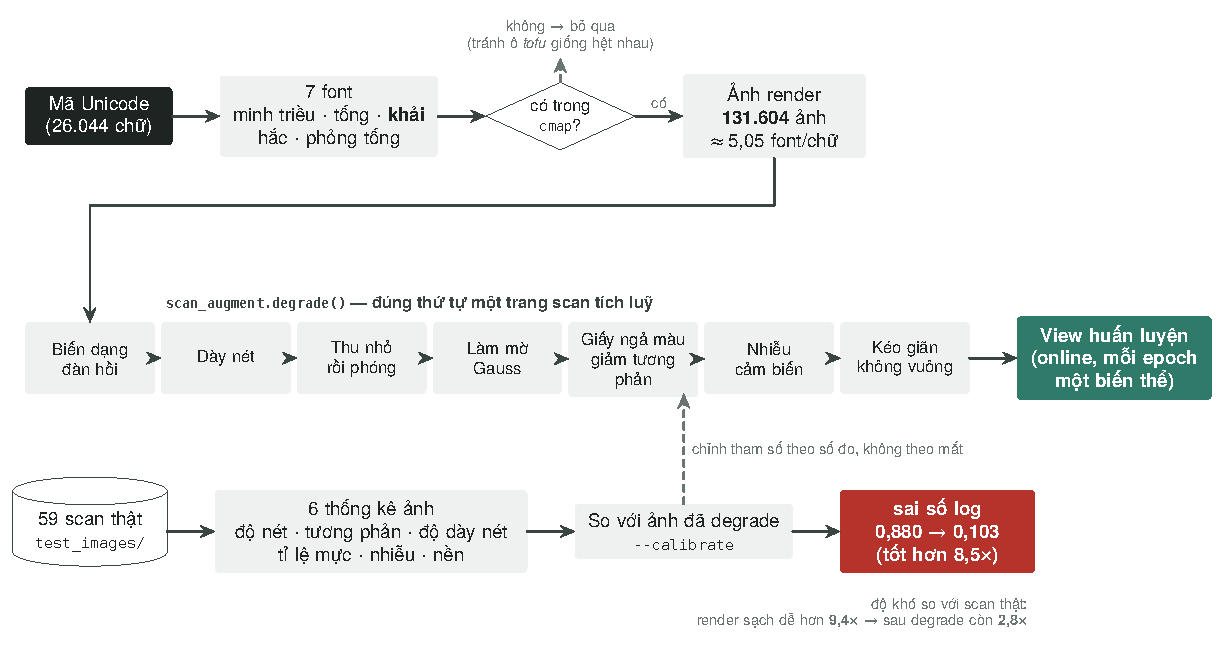
\includegraphics[width=\textwidth]{diagrams/d3-synthesis.pdf}
\caption{Sinh cặp dương. Mỗi mã Unicode được render qua những font có chứa nó trong \code{cmap}, rồi
đi qua \code{degrade()} theo thứ tự một trang scan bị suy giảm. Tham số được hiệu chỉnh dựa trên sáu
chỉ số đo từ 59 ảnh scan thật (Bảng~\ref{tab:degrade}).}
\label{fig:synthesis}
\end{figure*}

\begin{table}[t]
\caption{Khác biệt đo được giữa ảnh scan thật và ảnh render. Hàm suy giảm mô phỏng đúng sáu chỉ số này.}
\label{tab:degrade}
\centering\footnotesize
\begin{tabular}{@{}lrrrl@{}}
\toprule
Chỉ số & Scan & Render & Tỉ lệ & Ý nghĩa \\
\midrule
edge     & 15,6 & 102,3 & 0,15$\times$ & scan mờ hơn nhiều \\
contrast & 91,6 & 232,8 & 0,39$\times$ & mực xám nhạt \\
thick    & 0,051 & 0,028 & 1,82$\times$ & nét scan dày gấp đôi \\
fill     & 0,349 & 0,206 & 1,69$\times$ & do nét dày hơn \\
noise    & 10,1 & 2,7   & 3,77$\times$ & hạt nhiễu giấy \\
bg       & 254,0 & 255,0 & $\approx$1$\times$ & nền giấy hơi ngà \\
\bottomrule
\end{tabular}
\end{table}

Phần chênh 2,8 lần còn lại đến từ khác biệt về \textbf{nét chữ}: bút lông, các nét viết liền nhau,
tỉ lệ giữa các bộ phận bị lệch, có nét bị lược bớt. Những khác biệt này không thể tạo ra từ ảnh chữ in
chỉ bằng xử lý ảnh.

\subsection{Fine-tune}
\label{sec:ft}

Mục tiêu là dạy mô hình \textbf{không phụ thuộc vào kiểu chữ}: cùng một mã Unicode, dù viết bằng font
nào, cũng phải ra cùng một vector. Nhãn duy nhất là mã Unicode. Nhóm cố ý không dùng \code{RADICAL}
hay \code{STROKE\_NUM}, vì nếu huấn luyện trên bộ thủ rồi lại chấm điểm bằng chỉ số bộ thủ thì chỉ là
đo lại dữ liệu huấn luyện. Hình~\ref{fig:finetune} vẽ vòng huấn luyện và vòng đánh giá chạy song song.

\begin{figure*}[t]
\centering
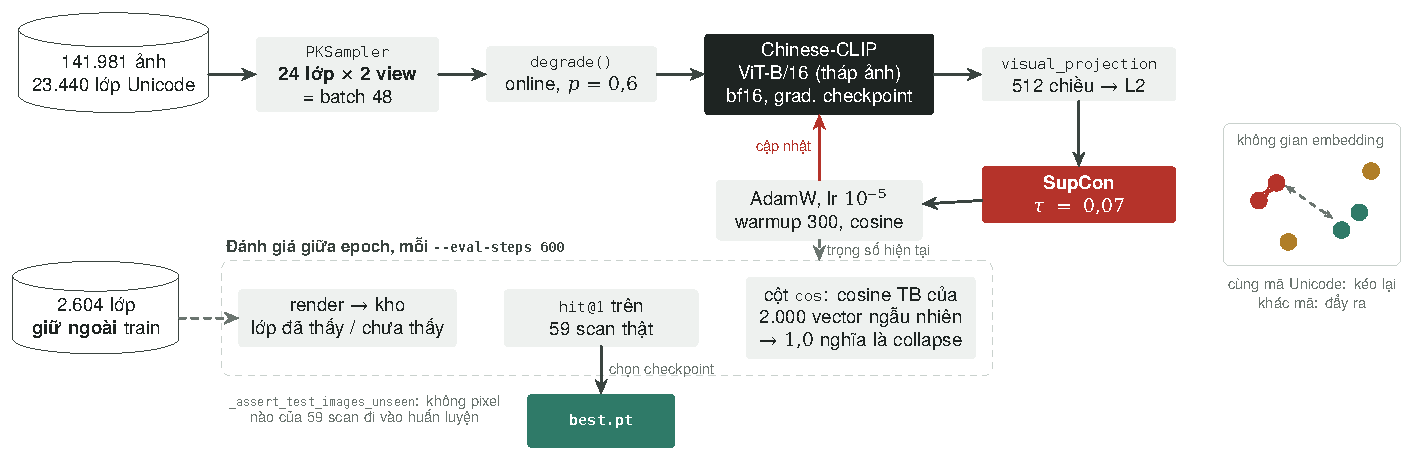
\includegraphics[width=\textwidth]{diagrams/d4-finetune.pdf}
\caption{Quá trình fine-tune. Mỗi batch gồm 24 lớp, mỗi lớp 2 ảnh; ảnh được làm suy giảm ngay khi nạp;
hàm mất mát là SupCon. Trong lúc huấn luyện, nhóm theo dõi \code{hit@1} trên ảnh scan thật, kết quả
trên lớp đã thấy và chưa thấy, và cột \code{cos} để phát hiện sớm khi biểu diễn bị hỏng.}
\label{fig:finetune}
\end{figure*}

\begin{table}[t]
\caption{Cấu hình fine-tune.}
\label{tab:ft}
\centering\footnotesize
\begin{tabular}{@{}p{1.6cm}p{6.0cm}@{}}
\toprule
Thành phần & Lựa chọn \\
\midrule
Backbone & Chinese-CLIP ViT-B/16, giữ nguyên \code{visual\_projection} (512 chiều) \\
Hàm mất mát & SupCon~\cite{supcon}, nhiệt độ 0,07 \\
Lấy mẫu & \textbf{P$\times$K: 24 lớp $\times$ 2 view mỗi batch} \\
Dữ liệu & 141.981 ảnh / 23.440 lớp \\
Suy giảm & \code{degrade()} chạy \textbf{trực tuyến} trong DataLoader, $p = 0{,}6$ \\
Tối ưu & AdamW, lr $10^{-5}$, warmup 300, cosine, bf16 \\
Chi phí & \textbf{3,7\,GB VRAM}, $\sim$4 phút/epoch, 6 epoch \\
\bottomrule
\end{tabular}
\end{table}

Công thức hàm mất mát và cách lấy mẫu được viết đầy đủ ở mục~\ref{sec:loss}. Trong
Bảng~\ref{tab:ft} có hai lựa chọn mà thiếu thì mô hình không học được, và cả hai đều rút ra từ lần
thất bại ở mục~\ref{sec:collapse}:

\begin{itemize}
  \item \textbf{Lấy mẫu theo P$\times$K.} Nếu rút ngẫu nhiên 48 ảnh từ 23.440 lớp, trung bình mỗi batch
        chỉ có khoảng 0,05 cặp cùng lớp. Gần như batch nào cũng không có cặp dương, và hàm mất mát
        không học được gì.
  \item \textbf{Dùng SupCon thay cho ArcFace.} Hàm mất mát SupCon không có tham số cần học, nên không
        có lớp nào khởi tạo ngẫu nhiên đẩy nhiễu ngược vào backbone.
\end{itemize}

Ảnh được làm suy giảm ngay lúc nạp dữ liệu chứ không render sẵn ra đĩa. Bộ sinh số ngẫu nhiên được
gieo theo (seed, epoch, chỉ số ảnh), nên mỗi epoch mỗi ảnh có một biến thể khác nhưng vẫn tái lập
được, và không tốn thêm dung lượng đĩa.

\subsection{Hàm mất mát và cách lấy mẫu}
\label{sec:loss}

Gọi $B$ là batch, $z_i = f_\theta(x_i)/\lVert f_\theta(x_i)\rVert_2$ là vector đã chuẩn hoá,
$y_i$ là mã Unicode của ảnh $x_i$, và $\tau = 0{,}07$. Đặt $P(i) = \{p \in B : y_p = y_i,\, p \neq
i\}$ là tập các ảnh cùng lớp với ảnh $i$. Hàm mất mát SupCon~\cite{supcon} là

\begin{equation}
\label{eq:supcon}
\mathcal{L} = \frac{1}{|A|}\sum_{i \in A}
\frac{-1}{|P(i)|}\sum_{p \in P(i)}
\log \frac{\exp(z_i^{\!\top} z_p/\tau)}
          {\displaystyle\sum_{a \in B \setminus \{i\}} \exp(z_i^{\!\top} z_a/\tau)},
\end{equation}

trong đó $A = \{i \in B : |P(i)| > 0\}$. Nói đơn giản, hàm này kéo các ảnh cùng chữ lại gần nhau và
đẩy các ảnh khác chữ ra xa. Khi cài đặt, có ba chi tiết không nhìn thấy trong công thức nhưng quyết
định việc nó có chạy đúng hay không:

\begin{enumerate}
  \item \textbf{Mẫu số không tính chính ảnh $i$}, nên phải che đường chéo của ma trận tương đồng.
        Cách thường dùng là gán $-\infty$ trước khi tính \code{logsumexp}.
  \item \textbf{$-\infty \cdot 0 = \mathrm{NaN}$.} Sau \code{logsumexp}, đường chéo vẫn là
        $-\infty$; nhân với mặt nạ dương (bằng 0 ở đường chéo) sẽ ra NaN, và toàn bộ gradient thành
        NaN ngay bước đầu. Phải gán đường chéo về 0 trước khi nhân mặt nạ. Nhóm đã thực sự gặp lỗi
        này.
  \item \textbf{Ảnh không có cặp dương phải bị loại khỏi phép lấy trung bình}, không phải tính là 0.
        Nếu tính là 0, giá trị hàm mất mát sẽ thay đổi tuỳ theo trong batch có bao nhiêu lớp lẻ.
\end{enumerate}

Khi biểu diễn bị hỏng hoàn toàn (mọi $z_i$ trùng nhau), \eqref{eq:supcon} có giá trị
$\ln(PK - 1) = \ln 47 \approx 3{,}85$. Biết trước con số này thì chỉ cần nhìn hàm mất mát là phát
hiện được sự cố.

\medskip
Cách lấy mẫu được viết thành một \code{Sampler} riêng thay vì trộn ngẫu nhiên:

{\footnotesize\ttfamily\raggedright
\textbf{Thuật toán 1: PKSampler}(nhãn, batch$=48$, K$=2$)\\
1\ \ P $\leftarrow$ max(2, batch // K)\ \ \ \ \# 24 lớp mỗi batch\\
2\ \ bỏ mọi lớp có $<$ K ảnh\ \ \ \ \ \ \ \# không dựng nổi cặp dương\\
3\ \ lặp mỗi epoch:\\
4\ \ \ \ \ hoán vị ngẫu nhiên danh sách lớp\\
5\ \ \ \ \ với mỗi khối P lớp liên tiếp:\\
6\ \ \ \ \ \ \ \ với mỗi lớp trong khối:\\
7\ \ \ \ \ \ \ \ \ \ \ lấy K ảnh, không lặp trong epoch\\
8\ \ \ \ \ \ \ \ trả về P$\cdot$K chỉ số làm một batch\\
}

\medskip
Lý do bước 1 và 2 là bắt buộc: với $C = 23.440$ lớp và batch ngẫu nhiên cỡ $B = 48$, số cặp dương
trung bình trong một batch là

\begin{equation}
\label{eq:pairs}
\mathbb{E}[\#\text{cặp dương}] = \binom{B}{2}\Pr[y_i{=}y_j] \approx 1128 \cdot \frac{1}{23.440}
\;\approx\; 0{,}05 .
\end{equation}

Tức là khoảng 95\% số batch không có cặp dương nào. Với những batch đó, \eqref{eq:supcon} không có
số hạng nào, hàm mất mát là hằng số và gradient bằng không. Đổi hàm mất mát không giải quyết được
chuyện này, vì lỗi nằm ở cách lấy mẫu.

% =====================================================================
\section{Phương pháp đánh giá}
\label{sec:eval}

Nhóm dành nhiều thời gian cho phần đánh giá, vì nếu chỉ số sai thì các kết luận phía sau cũng sai
theo. Có ba mức đánh giá, độ tin cậy tăng dần:

\begin{itemize}
  \item \textbf{Chỉ số gián tiếp (proxy)} trên toàn kho: \code{radical@k}, \code{stroke\_mae@k},
        \code{ids\_jaccard@k}. Các chỉ số này rẻ, chạy được trên cả 26.044 chữ, nhưng chỉ là nhãn yếu.
  \item \textbf{Nhãn thật lấy từ tên file} trên 59 ảnh scan. Ở mức này, đoán ngẫu nhiên đúng ở vị trí
        đầu tiên với xác suất khoảng $4{,}7\cdot10^{-4}$.
  \item \textbf{Nhãn do người gán} cho Phần 2, đã gán đủ 59/59 ảnh.
\end{itemize}

Cột \code{confidence} trong bảng nhãn là \textbf{đánh giá của người xem ảnh}, không lấy từ điểm số
của mô hình. Nhóm làm vậy có chủ ý: khi kiểm tra độ nhạy, nhóm lọc ra các nhãn chắc chắn bằng cột này
rồi chấm lại mô hình. Nếu \code{confidence} lấy từ điểm của mô hình thì phép kiểm tra đó thành dùng
mô hình để chấm chính nó. Có ba mức: \emph{high} (nhìn rõ nét quyết định), \emph{med} (còn một biến
thể rất giống, chỉ khác ở chỗ ảnh bị mờ) và \emph{low} (phải dựa vào ngữ cảnh nhiều hơn hình). Kết
quả cuối cùng là 53 high, 4 med, 2 low.

Các ảnh scan là những câu mở đầu \emph{Truyện Kiều}. Vì vậy nhóm gán nhãn bằng cách so hình trước,
rồi đối chiếu với cách viết chữ Nôm phổ biến của tác phẩm. \textbf{Khi hình và ngữ cảnh không khớp
thì nhóm theo hình}, và hạ \code{confidence} xuống \emph{med}. Ví dụ, bản scan viết ``qua'' là
\nom{戈} chứ không phải \nom{過}, viết ``năm'' là \nom{𢆥} chứ không phải \nom{年}.

\subsection{Định nghĩa chỉ số}

Với $N$ truy vấn, gọi $r_q$ là thứ hạng (tính từ 1) của ứng viên đúng đầu tiên cho truy vấn $q$; nếu
không có ứng viên đúng nào trong danh sách thì quy ước $1/r_q = 0$.

\begin{align}
\text{hit@}k &= \frac{1}{N}\sum_{q=1}^{N} \mathbf{1}[\,r_q \leq k\,],
& \text{MRR} &= \frac{1}{N}\sum_{q=1}^{N} \frac{1}{r_q}.
\end{align}

Nói cách khác, \code{hit@1} là tỉ lệ ảnh mà chữ đúng nằm ở vị trí đầu tiên, còn MRR thưởng thêm cho
những ảnh mà chữ đúng nằm ở vị trí gần đầu. \code{radical@k} là chỉ số gián tiếp: tỉ lệ trong $k$ ứng
viên đầu có cùng bộ thủ với truy vấn, lấy trung bình trên mọi truy vấn. Chỉ số này không cần nhãn
thật nên chạy được trên toàn kho, nhưng cũng vì vậy mà nó có giới hạn riêng, được đo ở
mục~\ref{sec:neg}.

Khoảng tin cậy được tính theo công thức Wilson~\cite{wilson} chứ không theo xấp xỉ chuẩn (Wald). Với
$\hat{p}$ là tỉ lệ đo được, $n$ là cỡ mẫu và $z = 1{,}96$:

\begin{equation}
\label{eq:wilson}
\frac{\hat{p} + \dfrac{z^2}{2n} \pm z\sqrt{\dfrac{\hat{p}(1-\hat{p})}{n} + \dfrac{z^2}{4n^2}}}
     {1 + \dfrac{z^2}{n}} .
\end{equation}

Lý do chọn Wilson: với $n = 59$ và tỉ lệ nhỏ như ở mô hình zero-shot ($\hat{p} = 0{,}0847$), công
thức Wald cho cận dưới âm, điều vô lý với một tỉ lệ. Khoảng Wilson luôn nằm trong $[0,1]$.

\textbf{Mọi tỉ lệ trong báo cáo đều kèm khoảng tin cậy 95\%}~\cite{wilson}. Với $n = 59$ và
$p \approx 0{,}5$, khoảng này rộng khoảng $\pm13$ điểm, nên mọi chênh lệch nhỏ hơn khoảng 15 điểm đều
không đủ để kết luận. Đây là giới hạn của tập test hiện có. Nhóm áp dụng nhất quán quy tắc này, và
trong cả đồ án chỉ có một so sánh vượt qua được ngưỡng đó.

% =====================================================================
\section{Kết quả}

\subsection{So sánh các backend trên toàn kho}

\begin{table}[t]
\caption{Toàn bộ kho 26.044 glyph, top-$K$ = 20. In đậm là giá trị tốt nhất mỗi cột.}
\label{tab:backend}
\centering\footnotesize
\begin{tabular}{@{}lrrrr@{}}
\toprule
Backend & radical@k $\uparrow$ & stroke $\downarrow$ & ids @k $\uparrow$ & img/s \\
\midrule
\code{resnet18} (gốc)      & 0,2316 & 2,8942 & 0,1031 & \textbf{3950} \\
\code{resnet18-gray}       & 0,2202 & 2,5658 & 0,1020 & 3937 \\
\code{chinese-clip} B/16   & 0,4843 & 2,6296 & 0,1997 & 358 \\
\code{chinese-clip-large}  & \textbf{0,5361} & 2,6992 & 0,2113 & 354 \\
\code{chinese-clip-huge}   & 0,5147 & 2,6547 & \textbf{0,2144} & 283 \\
\code{dinov2}              & 0,3081 & \textbf{2,3397} & 0,1251 & 306 \\
\bottomrule
\end{tabular}
\end{table}

Bảng~\ref{tab:backend} cho thấy Chinese-CLIP tốt hơn hẳn: \code{radical@k} gấp 2,31 lần bản gốc và
\code{ids\_jaccard} gấp 2,05 lần, trong khi tốc độ gần như không đổi giữa bản base và large (358 và
354 ảnh/giây). DINOv2 kém hơn ở bộ thủ nhưng lại tốt nhất về số nét, và chỉ trùng 12,9\% kết quả
top-$k$ với các mô hình CLIP. Vì vậy DINOv2 không hẳn là kém hơn, mà mạnh ở một khía cạnh khác.

\subsection{Giới hạn của chính chỉ số gián tiếp}

Thầy có đặt câu hỏi: \code{radical@k} dừng ở khoảng 0,5 có phải là đã bão hoà? Nhóm kiểm tra giả
thuyết ``top-$k$ quá ít nên không chứa đủ chữ cùng bộ thủ'' và thấy giả thuyết này sai: mức tối đa có
thể đạt của \code{radical@20} là 0,9862, chỉ 3\% truy vấn bị giới hạn bởi kích thước top-$k$. Ngoài
ra \code{radical@1} cũng chỉ đạt 0,6331, nên chỗ yếu nằm ngay ở láng giềng gần nhất chứ không ở cuối
danh sách.

Phép kiểm tra này cho thấy một điều quan trọng hơn: \textbf{\code{RADICAL} không hoàn toàn là thông
tin về hình dạng.} Chỉ 56,7\% ký tự thực sự chứa bộ thủ của nó trong hình chữ; số còn lại được xếp
vào bộ thủ đó vì lý do từ nguyên hoặc quy ước tra cứu. Ngay cả một phương pháp biết trước cách phân rã
chữ (oracle) cũng chỉ đạt \code{radical@20} = 0,7338. So với mức đó, \code{chinese-clip-large}
(0,5361) đã đạt khoảng 73\%, và gấp 24,4 lần mức ngẫu nhiên. Như vậy chỉ số chưa bão hoà, nhưng cũng
không nên cố tối ưu tiếp một chỉ số mà bản thân nó chỉ phản ánh đúng khoảng hai phần ba.

\subsection{Kết quả trên ảnh scan thật}
\label{sec:real}

\begin{figure}[t]
\centering
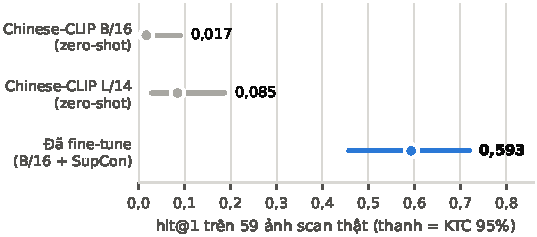
\includegraphics[width=\columnwidth]{figs/fig1-headline.pdf}
\caption{Kết quả chính: \code{hit@1} khi tìm trên toàn bộ 26.044 ký tự, đo trên 59 ảnh scan thật.
Thanh ngang là khoảng tin cậy 95\%. Khoảng tin cậy của bản zero-shot và bản fine-tune không chồng lên
nhau, nên đây là so sánh duy nhất trong đồ án mà 59 ảnh đủ để kết luận.}
\label{fig:headline}
\end{figure}

Đây là phép đo duy nhất không dùng chỉ số gián tiếp, và là con số nên dùng để đánh giá đồ án. Không
ảnh nào trong \code{test\_images/} được dùng để huấn luyện; điều này được kiểm tra bằng một lệnh
\code{assert} chạy trước mỗi lần huấn luyện.

Theo Hình~\ref{fig:headline}, bản fine-tune đạt \code{hit@1} = 0,5932 $[0{,}457; 0{,}719]$, so với
0,0847 $[0{,}028; 0{,}187]$ của \code{chinese-clip-large} zero-shot, tức 35/59 ảnh so với 5/59 ảnh,
cao hơn mức ngẫu nhiên khoảng 1.250 lần. \code{hit@10} đạt 0,7966 và MRR đạt 0,6691.

Trước khi fine-tune, kết quả thấp chủ yếu vì \textbf{ảnh truy vấn khác xa ảnh trong kho}, chứ không
phải vì mô hình yếu. Dấu hiệu rõ nhất là cùng một ký tự \nom{攅} được trả về ở vị trí đầu cho sáu ảnh
truy vấn khác nhau. Ảnh truy vấn là chữ viết tay trên giấy scan mờ, còn ảnh trong kho là chữ in khải
thư. Nhóm đã thử chuẩn hoá hình học (cắt sát phần mực, đệm thành ảnh vuông), nhưng kết quả chỉ thay
đổi trong phạm vi nhiễu. Khác biệt về hình học có thật, nhưng không phải nguyên nhân chính.

\begin{table}[t]
\caption{Phần 2: xếp hạng trong nhóm chữ cùng âm Quốc Ngữ, $n = 59$.}
\label{tab:part2}
\centering\footnotesize
\begin{tabular}{@{}lrrl@{}}
\toprule
Phương pháp & Đúng top-1 & MRR & KTC 95\% \\
\midrule
Chọn ngẫu nhiên trong nhóm & 0,1987 & --- & --- \\
\code{histogram} (bản gốc) & 0,4407 & 0,6070 & [0,312; 0,576] \\
\code{embedding} zero-shot & 0,4746 & 0,6566 & [0,343; 0,609] \\
\textbf{\code{embedding} fine-tune} & \textbf{0,8136} & \textbf{0,8983} & \textbf{[0,691; 0,903]} \\
\bottomrule
\end{tabular}
\end{table}

Bảng~\ref{tab:part2} là kết quả Phần 2. Khi chỉ xét 53 nhãn \emph{high}, bản fine-tune đạt 0,8491 so
với 0,4717 của histogram, nên kết luận không phụ thuộc vào sáu nhãn \emph{med}/\emph{low}.

Kết quả này cũng làm thay đổi một nhận định trước đó của nhóm. Với mô hình zero-shot, embedding chỉ
hơn histogram hai ảnh trên 59, nằm trong phạm vi nhiễu, nên lúc đó nhóm chỉ có thể khuyên dùng
embedding vì điểm số của nó hợp lý hơn, chứ chưa thể dựa vào độ chính xác. Sau fine-tune, khoảng cách
là 22 ảnh và hai khoảng tin cậy tách hẳn nhau, nên độ chính xác đã đủ làm căn cứ.

\subsection{Mô hình có chỉ học thuộc 23.440 chữ không?}
\label{sec:gen}

\begin{figure}[t]
\centering
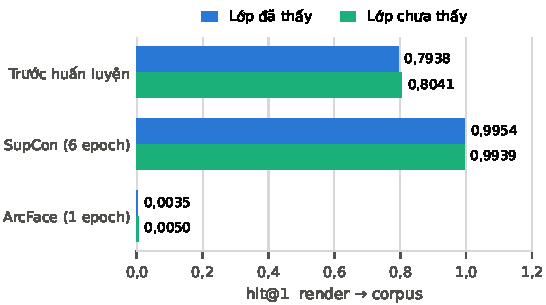
\includegraphics[width=\columnwidth]{figs/fig3-generalisation.pdf}
\caption{Kiểm tra khả năng tổng quát. 2.604 mã Unicode bị loại \emph{toàn bộ ảnh} khỏi tập huấn luyện
(chia theo lớp, không chia theo ảnh). Sau SupCon, kết quả trên lớp chưa thấy bằng lớp đã thấy. ArcFace
giảm mạnh ở \emph{cả hai} nhóm, dấu hiệu của biểu diễn bị hỏng chứ không phải overfit.}
\label{fig:gen}
\end{figure}

Với một mức tăng lớn như vậy, câu hỏi đầu tiên sẽ là mô hình có chỉ nhớ các chữ đã gặp hay không, nên
nhóm chuẩn bị phép kiểm tra này ngay từ đầu. Nhóm chia theo lớp chứ không theo ảnh, vì nếu chia theo
ảnh thì lớp nào cũng xuất hiện ở cả hai phía và phép đo không còn ý nghĩa. Hai nhóm có cùng kích
thước 2.604 và được chọn ngẫu nhiên giống nhau. Nhóm không chọn theo thứ tự mã Unicode, vì như vậy sẽ
lệch về khối chữ phổ thông trong khi tập giữ lại trải đều cả khối mở rộng Ext-B.

Theo Hình~\ref{fig:gen}, lớp đã thấy đạt 0,9954 và lớp chưa thấy đạt 0,9939, gần như bằng nhau. Điều
này phù hợp với cách SupCon hoạt động: nó không lưu tâm của từng lớp nên không có gì để học thuộc. Thứ
mô hình học được là cách so sánh hai ảnh, và cách so sánh đó áp dụng được cho cả những chữ chưa gặp.

\subsection{Quan sát định tính}

\begin{figure}[t]
\centering
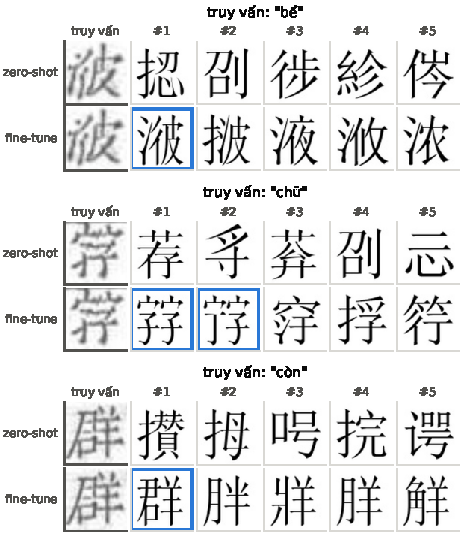
\includegraphics[width=\columnwidth]{figs/fig5-qualitative.pdf}
\caption{Năm kết quả đầu cho ba ảnh scan thật, trước và sau fine-tune. Khung xanh là ký tự đúng. Ảnh
truy vấn được chọn theo một quy tắc cố định (bản fine-tune đúng ở vị trí 1, bản zero-shot sai ở vị trí
1, lấy theo thứ tự tên file), không chọn ví dụ đẹp. Bản zero-shot trả về các chữ không liên quan về
cấu trúc; bản fine-tune trả về đúng chữ và các chữ cùng bộ.}
\label{fig:qual}
\end{figure}

Hình~\ref{fig:qual} cho thấy mô hình thực sự trả về những gì. Với truy vấn ``chữ'', bản fine-tune trả
về hai biến thể đúng ở hai vị trí đầu, cả hai đều có bộ phận \nom{字}, trong khi bản zero-shot trả về
những chữ chỉ giống ở độ dày đặc của nét.

% =====================================================================
\section{Kết quả âm}
\label{sec:neg}

Bốn kết quả dưới đây là những thử nghiệm không thành công hoặc giả thuyết bị bác bỏ. Nhóm vẫn ghi lại
vì đây là những hướng mà người làm tiếp rất dễ thử lại.

\subsection{Giả thuyết ``lỗi nằm ở \code{conv1}'' không đúng}

Bản gốc thay \code{conv1} bằng lớp một kênh khởi tạo ngẫu nhiên, tức bỏ đi bộ lọc tầng đầu đã được
pretrain. Nhóm nghĩ rằng chỉ cần sửa dòng này là đủ, nên làm thêm \code{resnet18-gray}: khởi tạo
\code{conv1} bằng tổng các bộ lọc RGB đã pretrain. Kết quả \code{radical@k} lại giảm nhẹ (0,2202 so với
0,2316). Như vậy sửa một dòng không cải thiện được ResNet18, và đây là lý do nhóm chuyển hẳn sang ViT
thay vì tiếp tục sửa baseline.

\subsection{Mô hình lớn hơn chưa chắc tốt hơn}

Từ base lên large, \code{radical@k} tăng 10,7\% tương đối, nhưng từ large lên huge lại giảm 4,0\%,
trong khi số chiều tăng 33\% và thời gian tăng 20\%. Điều này cho thấy tăng kích thước mô hình không
giúp được khi dữ liệu pretrain khác xa bài toán. Đây cũng là lý do nhóm chọn fine-tune thay vì chuyển
sang mô hình lớn hơn.

\subsection{ArcFace làm biểu diễn bị hỏng}
\label{sec:collapse}

\begin{figure}[t]
\centering
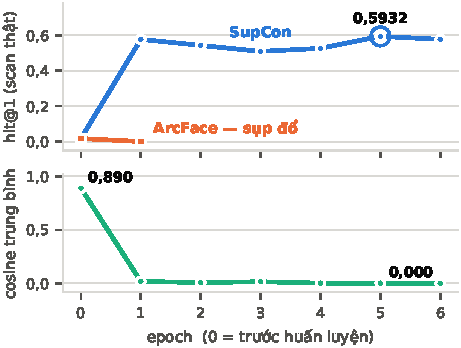
\includegraphics[width=\columnwidth]{figs/fig2-training.pdf}
\caption{Diễn biến huấn luyện. \emph{Trên}: \code{hit@1} trên ảnh scan thật qua từng epoch; với
ArcFace, mô hình mất hoàn toàn khả năng tìm kiếm sau một epoch. \emph{Dưới}: cosine trung bình giữa
2.000 vector ngẫu nhiên trong kho, dùng để phát hiện biểu diễn bị hỏng. Giá trị 0,890 ở zero-shot giải
thích vì sao mô hình ban đầu phân biệt kém; sau huấn luyện các vector tách nhau gần như vuông góc. Hai
đại lượng khác thang đo nên được vẽ ở hai khung riêng.}
\label{fig:train}
\end{figure}

Lần fine-tune đầu tiên dùng ArcFace~\cite{arcface} trên 23.440 lớp (scale 32, biên 0,30). Sau một
epoch, \code{hit@1} trên ảnh scan về 0, và kết quả tìm từ ảnh render sang kho giảm từ 0,79 xuống
0,0035 trên lớp đã thấy, từ 0,80 xuống 0,0050 trên lớp chưa thấy (Hình~\ref{fig:gen},
Hình~\ref{fig:train}).

Kết quả giảm ở \emph{cả hai} phía nên đây không phải overfit, mà là \textbf{biểu diễn bị hỏng}: mọi
ảnh bị dồn về gần cùng một vector. Nguyên nhân nằm ở dạng dữ liệu chứ không phải ở siêu tham số:
23.440 lớp nhưng mỗi lớp chỉ khoảng 6 ảnh. Lớp ArcFace khởi tạo ngẫu nhiên với 23.440 tâm không kịp
học được gì có ích, nên gradient nó truyền ngược về backbone gần như là nhiễu. Adam lại chuẩn hoá theo
độ lớn gradient, nên dù tốc độ học chỉ $10^{-5}$, trọng số vẫn thay đổi đủ để phá cấu trúc đã pretrain
trong khoảng 3.000 bước. Cắt chuẩn gradient cũng không giúp được, vì nhiễu sau khi cắt vẫn là nhiễu.

Sau lần này, nhóm thêm ba công cụ kiểm tra: (a) đánh giá ngay trong lúc chạy epoch, để phát hiện sự cố
sau khoảng một phút thay vì một giờ; (b) cột \textbf{cosine trung bình} ở Hình~\ref{fig:train}, tăng
dần về 1,0 khi biểu diễn bị hỏng. Không có cột này thì ``học chưa tốt'' và ``biểu diễn bị hỏng'' trông
giống nhau trên \code{hit@1}, trong khi hai trường hợp phải xử lý khác nhau; (c) biết trước rằng khi
SupCon bị hỏng, hàm mất mát sẽ đứng yên ở $\ln(P\!\cdot\!K - 1)$.

\subsection{Một nhãn gán sai làm giảm kết quả của chính nhóm}

\begin{figure}[t]
\centering
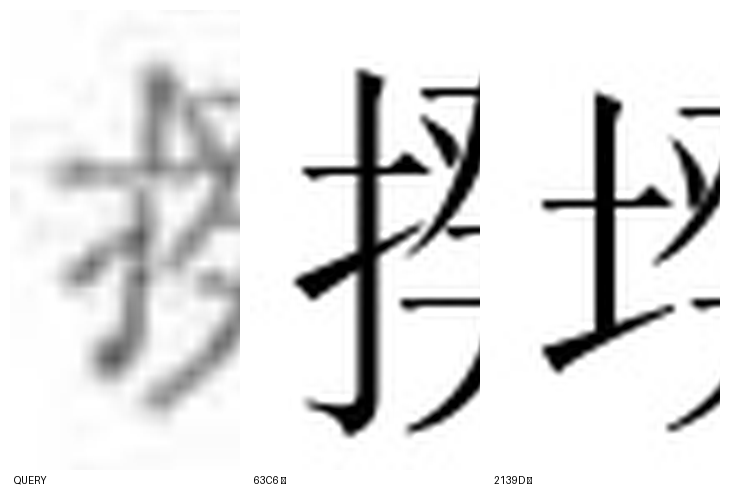
\includegraphics[width=0.62\columnwidth]{figs/coix-bo-trai.png}
\caption{Bộ bên trái của một ảnh scan, phóng to. Nét dọc dừng ở vạch ngang nên đây là \nom{土}, không
phải \nom{扌} (nét móc kéo xuống dưới vạch). Sửa nhãn này làm khoảng cách giữa hai phương pháp giảm từ
bốn ảnh xuống hai, tức là bất lợi cho kết luận mà nhóm đang muốn chứng minh.}
\label{fig:coix}
\end{figure}

Khi soát lại 11 dòng \emph{med}/\emph{low}, nhóm phát hiện một nhãn bị gán sai
(Hình~\ref{fig:coix}). Nhóm ghi lại để cho thấy với $n = 59$, chỉ một nhãn cũng đủ làm thay đổi kết
quả trong bảng.

% =====================================================================
\section{Xếp hạng lại bằng siêu dữ liệu}
\label{sec:rerank}

Ba cột \code{RADICAL}, \code{STROKE\_NUM} và \code{SHAPE\_MORPH} chứa những thông tin mà mô hình ảnh
không nhìn thấy trực tiếp. Câu hỏi đặt ra là: dùng chúng để \textbf{xếp hạng lại} danh sách ứng viên
mà mô hình ảnh trả về thì kết quả có tốt hơn không? Hiện tại câu trả lời là \emph{chưa}, và nhóm đã
tìm được nguyên nhân cụ thể. Hình~\ref{fig:rerankflow} vẽ thiết kế hai tầng.

\begin{figure*}[t]
\centering
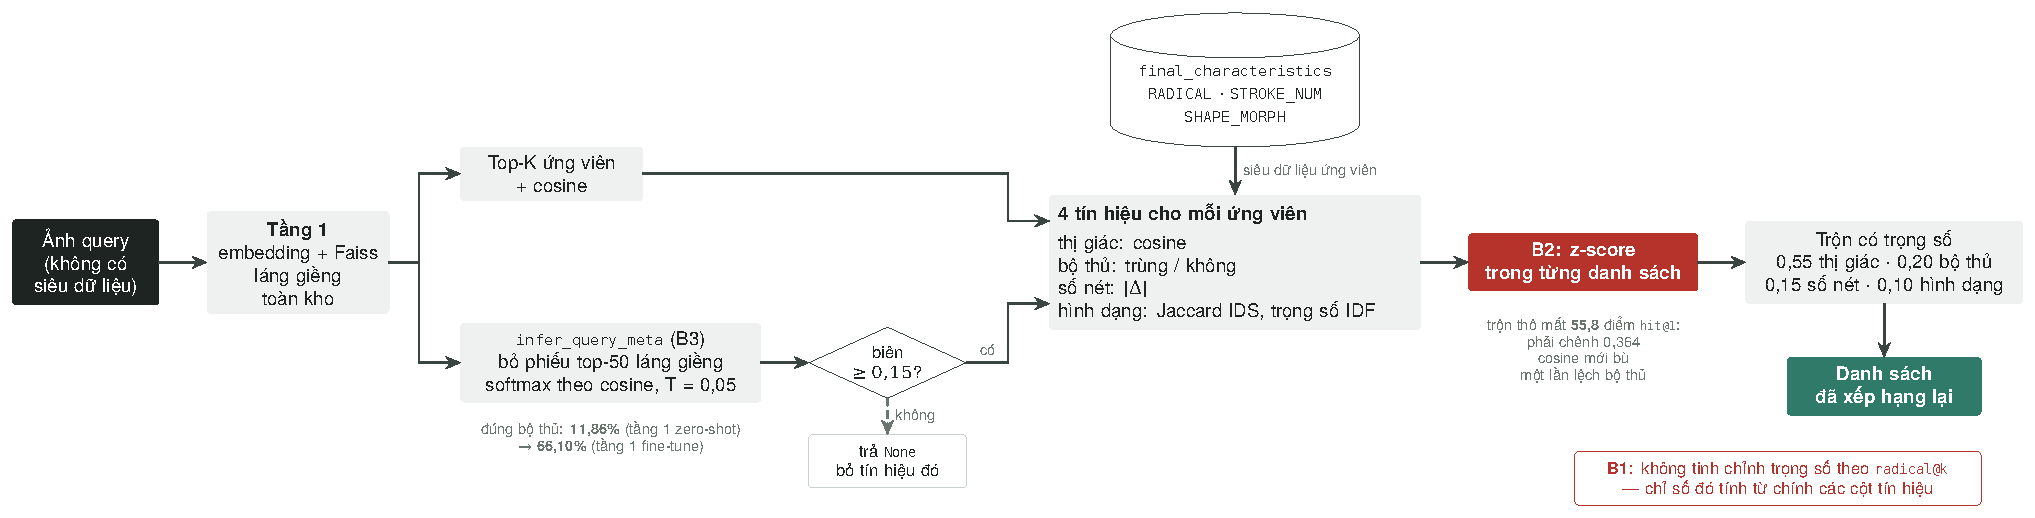
\includegraphics[width=\textwidth]{diagrams/d5-rerank.pdf}
\caption{Xếp hạng lại hai tầng. Ảnh truy vấn không có siêu dữ liệu nên phải suy ra bằng cách bỏ phiếu
từ các láng giềng gần nhất (B3). Bốn tín hiệu được chuẩn hoá z-score trong từng danh sách (B2) trước
khi cộng lại theo trọng số.}
\label{fig:rerankflow}
\end{figure*}

\begin{figure}[t]
\centering
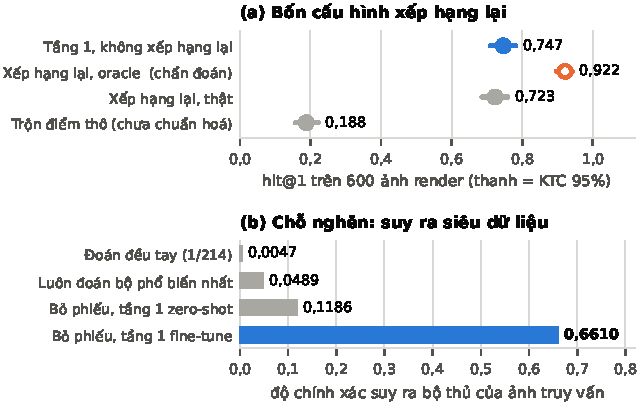
\includegraphics[width=\columnwidth]{figs/fig4-rerank.pdf}
\caption{(a) Bốn cấu hình xếp hạng lại trên 600 ảnh render, tầng 1 là \code{chinese-clip-large}. Cấu
hình oracle được vẽ rỗng vì nó \emph{cố ý} dùng siêu dữ liệu thật của truy vấn; đây là phép chẩn đoán
chứ không phải kết quả. (b) Độ chính xác khi suy ra bộ thủ của ảnh truy vấn, so với hai mức đoán.}
\label{fig:rerank}
\end{figure}

\subsection{Vì sao không dùng các chỉ số cũ để chấm}

Ba chỉ số gián tiếp được tính từ \emph{chính ba cột} mà tầng xếp hạng lại dùng làm đầu vào. Nếu chấm
bằng \code{radical@k} thì điểm sẽ tăng gần tới mức 0,978 nhưng không chứng minh được gì, vì mô hình đã
được cho sẵn đáp án. Để đo đúng, nhãn phải \textbf{độc lập} với ba cột đó. Nhóm dùng mã Unicode của
chính ký tự, trên tập ảnh render ($n = 600$, khoảng tin cậy khoảng $\pm3{,}5$ điểm).

\subsection{Ba nhận xét}

Từ Hình~\ref{fig:rerank}(a):

\begin{itemize}
  \item \textbf{Phải chuẩn hoá các tín hiệu trước khi cộng.} Cộng trực tiếp điểm thô làm \code{hit@1}
        giảm 56 điểm (0,7467 xuống 0,1883). Lý do là với trọng số mặc định, một ứng viên phải giống
        ảnh hơn tới 0,364 cosine mới bù được một lần khác bộ thủ, mà các ứng viên trong top-20 không
        bao giờ chênh nhau nhiều như vậy. Kết quả là danh sách bị sắp theo bộ thủ trước, rồi đến số
        nét, còn độ giống về hình chỉ còn dùng để phân xử khi hoà.
  \item \textbf{Siêu dữ liệu có thể giúp nhiều.} Cấu hình oracle tăng 17,5 điểm, nên bản thân ý tưởng
        không sai.
  \item \textbf{Nhưng hiện chưa khai thác được.} Cấu hình thực tế đạt 0,7233, hơi thấp hơn khi không
        xếp hạng lại.
\end{itemize}

\subsection{Chỗ nghẽn}

Ảnh truy vấn là ảnh scan chưa biết là chữ gì, nên không tra được siêu dữ liệu của nó. Nhóm thay bằng
cách \textbf{bỏ phiếu từ các láng giềng gần nhất}. Hình~\ref{fig:rerank}(b) đo riêng bước này: với
tầng 1 zero-shot, bỏ phiếu chỉ đoán đúng bộ thủ 11,86\%, hơn đoán mò 2,4 lần nhưng vẫn sai 88\% số
lần, trong khi bộ thủ chiếm trọng số 0,20 trong điểm tổng. Nói cách khác, tầng xếp hạng lại đang nhận
đầu vào phần lớn là sai.

Nguyên nhân là các phiếu được lấy từ láng giềng do tầng 1 trả về, mà tầng 1 zero-shot chỉ đúng 8,47\%
trên ảnh scan, nên phần lớn phiếu đến từ chữ sai. \textbf{Khi thay tầng 1 bằng mô hình đã fine-tune,
độ chính xác bỏ phiếu tăng lên 0,6610, gấp 5,6 lần.} Như vậy điểm yếu nằm ở tầng 1 đứng trước, không
nằm ở cách suy luận.

\subsection{Lưu ý về phép đo}

Tập ảnh render không dùng được để đánh giá mô hình đã fine-tune, vì đó chính là dữ liệu huấn luyện của
nó. Nhóm đã thử chỉ lấy 2.604 lớp giữ lại, rồi thử thêm trên ảnh đã suy giảm, nhưng cả hai đều cho kết
quả trên 0,98, không còn phân biệt được gì. Vì vậy phép đo ở trên chỉ áp dụng cho mô hình zero-shot.

% =====================================================================
\section{Thảo luận}
\label{sec:discuss}

Dưới đây là bốn điều nhóm rút ra trong quá trình làm đồ án. Chúng không chỉ đúng với chữ Nôm mà có thể
áp dụng cho các bài toán tương tự.

\subsection{Chỉ số đo được chưa chắc đã đo đúng}

\code{radical@k} rẻ, chạy được trên cả 26.044 ký tự và tăng đều khi đổi sang backbone tốt hơn, nên
trông như một chỉ số tốt. Nhưng mô hình đứng đầu theo chỉ số này chỉ đạt \code{hit@1} = 0,0847 trên
ảnh scan thật. Lý do không nằm ở sai số mà ở bản chất của chỉ số: hai chữ cùng bộ thủ có thể trông rất
khác nhau. Chỉ số gián tiếp vẫn cần cho giai đoạn sàng lọc, nhưng \textbf{cần đo giới hạn của nó
trước khi tin vào thứ hạng mà nó đưa ra}. Trong đồ án này, chỉ 59 ảnh có nhãn thật đã đủ để thay đổi
kết luận rút ra từ 26.044 ảnh có nhãn yếu.

\subsection{Lỗi ở khâu lấy mẫu dễ bị nhầm thành lỗi ở hàm mất mát}

Khi lần huấn luyện bằng ArcFace bị hỏng, phản xạ đầu tiên là đổi hàm mất mát, giảm tốc độ học, cắt
gradient. Không cách nào hiệu quả, vì nguyên nhân thật nằm ở cấu trúc batch (phương
trình~\eqref{eq:pairs}). Có một dấu hiệu chung để phân biệt: \textbf{nếu kết quả giảm cả trên lớp đã
thấy lẫn lớp chưa thấy thì đó là biểu diễn bị hỏng, không phải overfit}, vì overfit thì kết quả trên
tập huấn luyện vẫn tăng. Thêm một dòng tính cosine trung bình giữa các cặp ngẫu
nhiên~\cite{alignuniform} vào vòng đánh giá là đủ phát hiện chuyện này trong khoảng một phút, gần như
không tốn thêm gì.

\subsection{Một kết quả âm cần đi kèm mức tối đa có thể đạt}

Tầng xếp hạng lại không cải thiện kết quả. Nhưng chỉ nói ``không hiệu quả'' thì chưa đủ: có thể tín
hiệu không có ích, có thể cài đặt sai, cũng có thể chưa chỉnh tham số. Phép đo oracle (giả sử biết
đúng siêu dữ liệu của truy vấn) giúp tách các khả năng này: nếu biết đúng thì tăng 17,5 điểm, còn bước
suy ra siêu dữ liệu từ ảnh chỉ đúng 11,86\%. Kết luận vì vậy chuyển từ ``hướng này không dùng được''
thành ``hướng này còn nhiều dư địa, và cần sửa bước suy ra bộ thủ'', tức là biết được bước tiếp theo
cần làm gì.

\subsection{Khoảng tin cậy quyết định kết luận nào được phép viết}

Với $n = 59$, khoảng tin cậy 95\% rộng khoảng $\pm13$ điểm. Áp dụng nhất quán ngưỡng này thì
\textbf{cả đồ án chỉ có một so sánh đủ cơ sở}: zero-shot so với fine-tune. Thứ hạng giữa các backbone,
chênh lệch giữa các epoch, các biến thể của tầng xếp hạng lại đều nằm trong nhiễu, và được báo cáo
đúng như vậy. Báo cáo vì thế có ít khẳng định mạnh hơn, nhưng những khẳng định còn lại thì đáng tin.

% =====================================================================
\section{Hạn chế}

\begin{itemize}
  \item \textbf{59 ảnh scan là toàn bộ dữ liệu thật hiện có} và là hạn chế lớn nhất. Ngoài
        mục~\ref{sec:real}, mọi so sánh khác đều nằm trong phạm vi nhiễu. Cần khoảng 150 ảnh để khoảng
        tin cậy thu hẹp còn $\pm8$ điểm.
  \item \textbf{Mô hình fine-tune mới chạy một lần với một seed.} Kết quả giữa các epoch dao động
        0,51--0,59, xấp xỉ mức nhiễu của phép đo, nên con số 0,5932 nên hiểu là ``khoảng 0,55''.
  \item \textbf{Backbone là ViT-B/16 chứ không phải large}, vì bản large không đủ bộ nhớ GPU để huấn
        luyện trên máy dùng chung. Chưa biết fine-tune bản large sẽ đạt bao nhiêu.
  \item \textbf{Tầng xếp hạng lại chưa được thử với tầng 1 tốt nhất.} Hình~\ref{fig:rerank} đo với
        tầng 1 zero-shot; bốn cấu hình chưa được chạy lại với tầng 1 đã fine-tune.
  \item Nhãn Phần 2 được gán bằng cách \textbf{so hình}, chưa có chuyên gia Hán-Nôm kiểm tra. Còn
        6/59 dòng ở mức \emph{med}/\emph{low}.
  \item Ảnh truy vấn là chữ viết tay trên giấy scan, ảnh trong kho là chữ in khải thư; mọi con số đều
        đo trên đúng cặp dữ liệu này.
  \item Độ chính xác của chỉ mục xấp xỉ~\cite{hnsw} mới chỉ đo ở $N = 26.044$. Với HNSW, con số này
        thường giảm khi $N$ tăng, nên 99,1\% không áp dụng cho kho một triệu chữ.
\end{itemize}

% =====================================================================
\section{Hướng phát triển}
\label{sec:future}

Mục~\ref{sec:discuss} nói về những gì nhóm học được; mục này nói về những việc chưa làm và chi phí ước
tính của từng việc. Các việc được sắp theo tỉ lệ giữa lợi ích kỳ vọng và công sức bỏ ra.

\subsection{Tăng số ảnh đánh giá trước khi cải tiến mô hình}

Việc nên làm trước tiên không nằm ở mô hình. Với $n = 59$, khoảng tin cậy Wilson ở $\hat{p} \approx
0{,}5$ rộng $\pm13$ điểm (mục~\ref{sec:eval}), nên mọi thay đổi nhỏ hơn 13 điểm đều chưa phân biệt
được với nhiễu. Nếu tăng lên khoảng 300 ảnh, khoảng này còn $\pm5{,}7$ điểm, đủ để đo những cải tiến
vài điểm, vốn là mức của hầu hết các ý tưởng còn lại trong mục này. Việc này chỉ cần công scan và gán
nhãn, không cần GPU.

Đi kèm là hai việc để nhãn đáng tin hơn: (i) cho \emph{hai} người gán nhãn Phần 2 độc lập rồi tính hệ
số đồng thuận Cohen $\kappa$, thay vì một người như hiện nay; (ii) nhờ người đọc được Hán-Nôm kiểm tra
lại 6/59 dòng \emph{med}/\emph{low}. Mục~\ref{sec:neg} đã cho thấy chỉ một nhãn sai cũng làm thay đổi
kết quả của nhóm.

\subsection{Chọn mẫu âm khó (hard negative mining)}

Nhật ký huấn luyện cho thấy hàm mất mát giảm còn 0,0068 chỉ sau khoảng 400 bước. Điều đó không có
nghĩa mô hình đã rất tốt, mà là các batch quá dễ: 24 lớp chọn ngẫu nhiên từ 23.440 lớp gần như chắc
chắn khác nhau cả về bộ thủ lẫn số nét, nên mô hình sớm không còn gì để học. Có hai cách sửa, đều không
cần đổi kiến trúc:

\begin{itemize}
  \item \textbf{Chọn mẫu âm theo bộ thủ.} Dùng cột bộ thủ có sẵn trong
        \code{final\_characteristics-v2.xlsx} để mỗi batch có nhiều lớp \emph{cùng} bộ thủ. Dữ liệu
        đã có, chỉ cần sửa \code{PKSampler} ở mục~\ref{sec:loss}.
  \item \textbf{Chọn mẫu âm khó vừa phải (semi-hard) trong lúc huấn luyện.} Sau mỗi epoch, tính lại
        vector của toàn kho bằng chính mô hình đang huấn luyện, rồi lấy $k$ láng giềng gần nhất của mỗi
        lớp làm mẫu âm cho epoch sau. Chi phí thêm là một lần tính vector cho 26.044 ảnh mỗi epoch,
        khoảng 71 giây với cấu hình ở Phụ lục~\ref{app:env}, nhỏ so với thời gian huấn luyện.
\end{itemize}

Cần nhớ cảnh báo ở mục~\ref{sec:collapse}: mẫu âm càng khó thì nguy cơ biểu diễn bị hỏng càng cao. Mọi
thử nghiệm theo hướng này đều phải theo dõi chỉ số \code{cos} (cosine trung bình của 2.000 vector ngẫu
nhiên) song song với hàm mất mát, vì khi biểu diễn bị hỏng, hàm mất mát \emph{cũng} có thể giảm.

\subsection{Thử backbone lớn hơn trong giới hạn bộ nhớ GPU}

Nhóm dừng ở ViT-B/16 vì ViT-L/14 không đủ bộ nhớ trên máy dùng chung, chứ không phải vì đã thấy bản
large kém hơn. Ở chế độ zero-shot, large \emph{có} tốt hơn base, nên câu hỏi này vẫn còn mở. Có ba
cách để chạy large trong cùng 6\,GB: dùng LoRA thay vì cập nhật toàn bộ trọng số, dùng gradient
checkpointing, và cộng dồn gradient qua nhiều bước để giữ nguyên batch hiệu dụng $P \times K = 24
\times 2$. Đồng thời nên chạy ba seed thay vì một, vì chênh lệch giữa các epoch (0,51--0,59) đã xấp
xỉ mức nhiễu.

\subsection{Dữ liệu viết tay thật}

Hiện tại mọi cặp dương đều được tạo bằng cách render font in rồi làm suy giảm cho giống ảnh scan
(mục~\ref{sec:render}). Cách này mô phỏng được ảnh hưởng của \emph{quá trình scan}, nhưng không mô
phỏng được \emph{nét bút}: tốc độ viết, mực nhoè, các nét viết liền. Vì vậy khoảng cách còn lại giữa
ảnh viết tay và chữ in trong kho không thể thu hẹp thêm chỉ bằng augment. Hướng đi là bổ sung ảnh chữ
viết bút lông thật, bằng cách tự thu thập hoặc dùng các bộ dữ liệu chữ Hán viết tay có sẵn rồi ánh xạ
sang ký tự Nôm qua mã Unicode.

\subsection{Hoàn thiện tầng xếp hạng lại}

Mục~\ref{sec:rerank} đã xác định chỗ nghẽn nằm ở bước suy ra bộ thủ của \emph{ảnh truy vấn}, không
phải ở cách cộng điểm. Oracle cho thấy còn khoảng 17,5 điểm nếu bước này đúng. Việc cụ thể là huấn
luyện một bộ phân loại bộ thủ trên chính kho ảnh đã có nhãn bộ thủ, rồi đưa xác suất của nó (thay vì
một nhãn duy nhất) vào công thức cộng điểm. Ngoài ra cần chạy lại cả bốn cấu hình ở
Hình~\ref{fig:rerank} với tầng 1 \emph{đã} fine-tune, vì phép đo hiện tại dùng tầng 1 zero-shot nên
chưa nói được gì về hệ thống cuối cùng.

\subsection{Kho lớn hơn}

Mọi kết luận về chỉ mục đều đo ở $N = 26.044$, khi \code{IndexFlatIP} vẫn là lựa chọn hợp lý vì việc
tìm kiếm chỉ chiếm 6\% thời gian. Khi kho lớn hơn cần kiểm tra lại hai điều: ngưỡng thực sự nên chuyển
sang chỉ mục xấp xỉ (ước tính hiện tại khoảng 300.000 ký tự là ngoại suy, chưa đo), và độ chính xác của
HNSW~\cite{hnsw} khi $N$ lớn, vì con số 99,1\% đo ở $N = 26.044$ không áp dụng cho một triệu chữ.

\subsection{Công bố tập ảnh scan}

59 ảnh scan có nhãn hiện là tập đánh giá thật duy nhất của đồ án. Theo hiểu biết của nhóm, chưa có bộ
dữ liệu công khai nào đúng dạng \emph{ảnh chữ Hán-Nôm viết tay $\rightarrow$ ký tự trong kho chữ in}.
Nếu mở rộng được lên vài trăm ảnh như đề xuất ở trên, việc công bố tập này kèm cách đánh giá và khoảng
tin cậy sẽ có ích cho người làm sau hơn cả các con số của đồ án. Tập hiện tại đã có trong kho mã nguồn
ghi ở đầu bài.

\begin{table}[h]
\caption{Các hướng phát triển, sắp theo tỉ lệ lợi ích trên chi phí.}
\label{tab:future}
\centering\footnotesize
\newcolumntype{L}[1]{>{\raggedright\arraybackslash}p{#1}}
\begin{tabular}{@{}L{2.5cm}L{1.75cm}L{3.3cm}@{}}
\toprule
Việc & Chi phí & Kỳ vọng \\
\midrule
$n$: 59 $\rightarrow$ 300 & gán nhãn & KTC $\pm13 \rightarrow \pm5{,}7$ điểm \\
Mẫu âm theo bộ thủ & sửa sampler & gradient không tắt sớm \\
Semi-hard mining & $+71$\,s/epoch & chưa rõ; phải theo dõi \code{cos} \\
ViT-L + LoRA & vừa 6\,GB & trả lời câu hỏi về kích thước \\
Ảnh bút lông thật & thu thập & thu hẹp khác biệt dữ liệu \\
Phân loại bộ thủ & huấn luyện phụ & tối đa $+17{,}5$ điểm (oracle) \\
\bottomrule
\end{tabular}
\end{table}

% =====================================================================
\section{Kết luận}

Mục~\ref{sec:discuss} đã nêu những bài học chung; phần này chỉ tóm tắt kết luận về chính hệ thống.
Môi trường và chi phí tính toán nằm ở Phụ lục~\ref{app:env}, cấu trúc gói nộp ở
Phụ lục~\ref{app:pkg} và Bảng~\ref{tab:pkg}.

\begin{enumerate}
  \item \textbf{Nên dùng Chinese-CLIP.} Tốt hơn ResNet18 2,31 lần ở \code{radical@k} mà gần như không
        tốn thêm thời gian. Không cần chuyển lên ViT-H vì bản lớn hơn không tốt hơn.
  \item \textbf{Fine-tune mang lại cải thiện lớn nhất.} \code{hit@1} trên ảnh scan thật tăng từ 0,0847
        lên 0,5932, Phần 2 tăng từ 0,4746 lên 0,8136, và mô hình không chỉ học thuộc các chữ đã gặp.
  \item \textbf{Giữ cách tìm kiếm chính xác} \code{IndexFlatIP} cho đến khi kho vượt khoảng 300.000 ký
        tự; ở kích thước hiện tại, tìm kiếm chỉ chiếm 6\% thời gian.
  \item \textbf{Xếp hạng lại bằng siêu dữ liệu chưa dùng được, nhưng đã rõ nguyên nhân.} Oracle cho
        thấy còn khoảng 17,5 điểm; chỗ cần sửa là bước suy ra bộ thủ của ảnh truy vấn.
  \item \textbf{Các việc tiếp theo} được liệt kê ở mục~\ref{sec:future} và Bảng~\ref{tab:future}. Ba
        việc nên làm trước là tăng số ảnh đánh giá, chọn mẫu âm theo bộ thủ, và bổ sung dữ liệu chữ
        viết bút lông thật, thứ mà render font không tạo ra được.
\end{enumerate}

% =====================================================================
\begin{thebibliography}{99}
\bibitem{chineseclip} A. Yang \emph{và cộng sự}, ``Chinese CLIP: Contrastive Vision-Language
Pretraining in Chinese,'' arXiv:2211.01335, 2022.
\bibitem{dinov2} M. Oquab \emph{và cộng sự}, ``DINOv2: Learning Robust Visual Features without
Supervision,'' arXiv:2304.07193, 2023.
\bibitem{resnet} K. He, X. Zhang, S. Ren và J. Sun, ``Deep Residual Learning for Image
Recognition,'' CVPR, 2016.
\bibitem{supcon} P. Khosla \emph{và cộng sự}, ``Supervised Contrastive Learning,'' NeurIPS, 2020.
\bibitem{arcface} J. Deng, J. Guo, N. Xue và S. Zafeiriou, ``ArcFace: Additive Angular Margin Loss
for Deep Face Recognition,'' CVPR, 2019.
\bibitem{faiss} J. Johnson, M. Douze và H. Jégou, ``Billion-scale similarity search with GPUs,''
IEEE Transactions on Big Data, 2019.
\bibitem{hnsw} Y. A. Malkov và D. A. Yashunin, ``Efficient and robust approximate nearest neighbor
search using Hierarchical Navigable Small World graphs,'' IEEE TPAMI, 2020.
\bibitem{wilson} E. B. Wilson, ``Probable Inference, the Law of Succession, and Statistical
Inference,'' J. Amer. Statist. Assoc., 1927.
\bibitem{clip} A. Radford \emph{và cộng sự}, ``Learning Transferable Visual Models From
Natural Language Supervision,'' ICML, 2021.
\bibitem{vit} A. Dosovitskiy \emph{và cộng sự}, ``An Image is Worth 16x16 Words: Transformers for
Image Recognition at Scale,'' ICLR, 2021.
\bibitem{facenet} F. Schroff, D. Kalenichenko và J. Philbin, ``FaceNet: A Unified Embedding for Face
Recognition and Clustering,'' CVPR, 2015.
\bibitem{intriplet} A. Hermans, L. Beyer và B. Leibe, ``In Defense of the Triplet Loss for Person
Re-Identification,'' arXiv:1703.07737, 2017.
\bibitem{infonce} A. van den Oord, Y. Li và O. Vinyals, ``Representation Learning with Contrastive
Predictive Coding,'' arXiv:1807.03748, 2018.
\bibitem{simclr} T. Chen, S. Kornblith, M. Norouzi và G. Hinton, ``A Simple Framework for Contrastive
Learning of Visual Representations,'' ICML, 2020.
\bibitem{moco} K. He, H. Fan, Y. Wu, S. Xie và R. Girshick, ``Momentum Contrast for Unsupervised
Visual Representation Learning,'' CVPR, 2020.
\bibitem{alignuniform} T. Wang và P. Isola, ``Understanding Contrastive Representation Learning
through Alignment and Uniformity on the Hypersphere,'' ICML, 2020.
\bibitem{synth90k} M. Jaderberg, K. Simonyan, A. Vedaldi và A. Zisserman, ``Synthetic Data and
Artificial Neural Networks for Natural Scene Text Recognition,'' NIPS Deep Learning Workshop, 2014.
\bibitem{synthtext} A. Gupta, A. Vedaldi và A. Zisserman, ``Synthetic Data for Text Localisation in
Natural Images,'' CVPR, 2016.
\bibitem{elastic} P. Y. Simard, D. Steinkraus và J. C. Platt, ``Best Practices for Convolutional
Neural Networks Applied to Visual Document Analysis,'' ICDAR, 2003.

\end{thebibliography}

% =====================================================================
\appendices
\section{Tái lập số liệu}

Mọi con số trong báo cáo đều sinh ra từ các lệnh dưới đây, chạy \textbf{từ thư mục gốc của dự án}, vì
các script tìm \code{./images}, \code{./output}, \code{./test\_images} theo thư mục hiện tại. Hình vẽ
sinh bằng \code{make\_figures.py}, sơ đồ sinh bằng \code{report/diagrams/build.sh}. Hướng dẫn đầy đủ,
kèm giá trị mong đợi sau mỗi bước và cách xử lý sự cố, nằm trong \code{README.md} của kho mã:
\url{https://github.com/vo-hoang-kh4ng/comparing-character-glyph-images-Sino-N-m}

{\footnotesize\ttfamily\raggedright
\# Đặt PY=.venv/bin/python cho gọn\\
PY=.venv/bin/python\\[4pt]
\# chuẩn bị: Python 3.10+, một GPU $\geq$ 6\,GB\\
python -m venv .venv\\
\$PY -m pip install -r requirements.txt\\
bash download\_fonts.sh\\[4pt]
\# so sánh backend (mục VI-A, VI-B)\\
\$PY search\_all\_chars\_in\_corpus.py \textbackslash\\
\hspace*{1em}--backend <backend> --device cuda\\
\$PY benchmark\_extractors.py\\
\$PY analyze\_metric\_ceiling.py\\
\$PY benchmark\_search.py\\[4pt]
\# sinh dữ liệu huấn luyện, rồi fine-tune (mục IV)\\
\$PY render\_fonts.py\\
\$PY scan\_augment.py --calibrate\\
\$PY finetune\_glyph.py --smoke\\
\$PY finetune\_glyph.py --epochs 6 --device cuda\\[4pt]
\# đánh giá trên scan thật (mục VI-C)\\
\$PY search\_all\_chars\_in\_corpus.py \textbackslash\\
\hspace*{1em}--backend chinese-clip-ft --device cuda\\
\$PY evaluate\_test\_images.py \textbackslash\\
\hspace*{1em}--backend chinese-clip-ft --device cuda \textbackslash\\
\hspace*{1em}--labels output/label\_sheets/labels.csv\\[4pt]
\# xếp hạng lại: bốn cấu hình (mục VIII)\\
\$PY -m pytest -q\\
S="--suite render --sample 600"\\
\$PY evaluate\_rerank.py \$S --no-rerank\\
\$PY evaluate\_rerank.py \$S --oracle-meta\\
\$PY evaluate\_rerank.py \$S\\
\$PY evaluate\_rerank.py \$S --normalize none\\[4pt]
\# hình vẽ và sơ đồ trong bài\\
\$PY make\_figures.py\\
bash report/diagrams/build.sh\\
}

{\sloppy Tên đầy đủ của file nhãn là \code{output/label\_sheets/label\_template.csv}; ở trên viết
tắt cho vừa cột.\par} Nhật ký huấn luyện đầy đủ, gồm cả lần ArcFace bị hỏng ở mục~\ref{sec:collapse},
nằm trong \code{output/finetune/train.log}.

\section{Môi trường và chi phí tính toán}
\label{app:env}

\begin{table}[h]
\caption{Môi trường đã chạy thử. Cột VRAM là mức dùng cao nhất đo được, không phải dung lượng card.}
\label{tab:env}
\centering\footnotesize
\begin{tabular}{@{}ll@{}}
\toprule
Thành phần & Giá trị \\
\midrule
GPU (huấn luyện) & NVIDIA H100 80\,GB, dùng tối đa \textbf{3,7\,GB} \\
CPU & Intel Xeon Platinum 8462Y+, 16 nhân \\
RAM & 188\,GB \\
Python & 3.10.12 \\
PyTorch & 2.6.0+cu124 \\
Transformers & 4.57.6 \\
Chỉ mục & Faiss \code{IndexFlatIP} (chính xác) \\
\bottomrule
\end{tabular}
\end{table}

Mức VRAM tối đa chỉ 3,7\,GB nhờ dùng \code{gradient\_checkpointing} và xoá hẳn phần xử lý văn bản sau
khi nạp mô hình. Bài toán chỉ dùng ảnh, nên \code{text\_model} và \code{text\_projection} không cần
thiết. Vì vậy \textbf{toàn bộ quá trình huấn luyện chạy được trên một GPU 6\,GB thông thường}, không
cần phần cứng như trong Bảng~\ref{tab:env}.

Về thời gian, đo trên cấu hình trên: render bảy font cho 26.044 ký tự mất khoảng 25 phút (chỉ chạy một
lần); mỗi epoch fine-tune khoảng 4 phút, 6 epoch khoảng 25 phút; tính lại vector cho toàn kho khoảng 3
phút; đánh giá 59 ảnh scan mất vài giây. Tức là \textbf{các kết quả chính có thể tái lập trong khoảng
một giờ}, chưa tính thời gian tải mô hình pretrain lần đầu.

Checkpoint fine-tune nặng 329\,MB ở fp32. Bản trên Hugging Face lưu ở fp16 (165\,MB). Việc này không
làm sai lệch kết quả, vì khi nạp mô hình, mã nguồn đã gọi \code{model.to(fp16)} ngay từ đầu. Nhóm đã
kiểm tra bằng cách so toàn bộ 26.044 vector của kho giữa hai bản: sai khác tuyệt đối lớn nhất là
$0{,}0$.

\section{Cấu trúc gói nộp}
\label{app:pkg}

Kho 26.044 ảnh và các bảng \code{.xlsx} là dữ liệu đề bài cho nên không đóng gói lại;
\code{data/DATA.md} ghi rõ tên file và vị trí cần đặt để các script chạy được. Bộ kiểm thử chạy bằng
\code{\$PY -m pytest -q}; khi thiếu các bảng \code{.xlsx} thì một số test sẽ được bỏ qua, đây là hành
vi đã định sẵn chứ không phải lỗi.

\begin{table}[h]
\caption{Nội dung \code{submission.zip}.}
\label{tab:pkg}
\centering\footnotesize
\newcolumntype{L}[1]{>{\raggedright\arraybackslash}p{#1}}
\begin{tabular}{@{}L{1.5cm}L{6.1cm}@{}}
\toprule
Thư mục & Nội dung \\
\midrule
\code{src/} & Toàn bộ mã nguồn của nhóm, kèm \code{requirements.txt} và bộ kiểm thử. \\
\code{data/} & 59 ảnh scan dùng để đánh giá, bảng nhãn, nhật ký huấn luyện, và \code{DATA.md} hướng dẫn
              lấy lại các bảng \code{.xlsx} gốc. \\
\code{model/} & \code{MODEL.md}: đường dẫn tải trọng số và đoạn mã nạp mô hình. Trọng số \textbf{không}
              nằm trong gói theo đúng yêu cầu; xem liên kết ở đầu bài. \\
\code{report/} & Báo cáo bản PDF và bản Doc, kèm \code{paper.tex} và thư mục \code{figs/}. \\
\bottomrule
\end{tabular}
\end{table}

\end{document}
